\documentclass[10pt,landscape,oneside]{book}
\usepackage{caption}
\usepackage{etoolbox}
\usepackage[final]{grffile}
\usepackage{graphicx}
\usepackage{fancyvrb}
\usepackage[T1]{fontenc}
\usepackage{fancyhdr}
\usepackage{listings}
\usepackage{calc}
\graphicspath{{/home/mkg/Dropbox/images/}}
\pagestyle{headings}
\usepackage{lipsum}
\usepackage[hidelinks=true,linktoc=all]{hyperref}
\urlstyle{same}
\usepackage[all]{hypcap}\begin{document}
\frontmatter
\title{Selected Photographs}
\author{Michael Gogins \\ \texttt{michael.gogins@gmail.com}}
%\subtitle{Volume I}
%\dedication{This book is for Mick.}
.
\newpage
\noindent This book is copyright 2019 by Michael Gogins, all rights reserved. The contents of this book are licensed under the terms of the Creative Commons \href{https://creativecommons.org/licenses/by-nc-nd/4.0/legalcode}{\textbf{Attribution-NonCommercial-NoDerivatives 4.0 International} } license. In short, you may use, print, and copy this book or any of its contents for your own personal use, but you may not use this book or any of its contents as part of your own projects, or for commercial purposes.

If you wish to use this book or any of its contents for your own projects, or for commercial purposes, for example to re-publish or to exhibit in a gallery, please contact me directly.
\maketitle

\tableofcontents
\listoffigures

\mainmatter
\pagestyle{headings}

\chapter{Introduction}

This book contains my selection of 500 pictures from a lifetime of taking photographs. I have never been a professional, but I was and still am committed to the art of photography. These pictures were variously taken with 35 mm film cameras, a variety of digital cameras, and smartphones. They were taken in ny native state of Utah, the state of Washington, California, New York, other states, and various countries around the world. 

I am a ``street photographer`` open to abstraction. I shoot what catches my eye and I prize beauty. When I take pictures of people, I often prefer they don't notice. My reason for doing photography is to see more clearly what God has created.

I have tended to use the sharpest possible camera that is small enough to carry with me at all times. For some years now I have been using the Sony RX100 series. Increasingly, however, I am finding that my smartphone is a real camera.

As the file size of this book would become unmanageable thanks to the use of uncompressed images, it has been split into a number of volumes. Even so, the files are huge. However, they do enable the reader to zoom into the images in full detail or to extract them for printing at high resolution.

If I take more pictures that I think are good enough to be in this book, I will add them, and remove as many that are not quite good enough, to keep the total at 500 pictures.

\chapter{Photographs}

These images are all in natural color. They are all shot as far as possible without image manipulation; in a few cases, I have leveled horizons or removed spots. I shoot in JPEG rather than RAW. Selected metadata from the photographs is printed. If the photograph is a digital scan of a 35 mm slide, the creation date is the date of that scan. Captions are sporadic and cryptic, to say the least.

All pictures are included in the full resolution with which they were taken. Thus, you can zoom into any image to see more detail. Pictures copied out of this book will also be in full resolution.

I invite the reader to copy pictures out of this book for printing and viewing, but not for commercial use or re-publication. 



\clearpage
\onecolumn
\noindent This is a scan of the first picture I took that I actually liked, a 35 mm slide. It was in 1968 in the back yard of my father's girlfriend Doreen's house in Taylorsville, Utah, just after sunset. I believe this was Christmas Day.
\begin{lstlisting}
Filename: c-2013-03-12_12-07-24.jpg

Date: 2013:03:12 12:07:26
\end{lstlisting}
\clearpage

\includegraphics[width=\linewidth,height=\textheight,keepaspectratio,bb= 0 0 93 62]{/home/mkg/Dropbox/images/c-2013-03-12_12-07-24.jpg}
\clearpage
\onecolumn
\noindent Scan of a slide of my grandfather Milton (Mick) Swensen, my sister Wendy, my grandmother Jane, and myself, Murray, Utah, Christmas or New Years 1968 I think.
\begin{lstlisting}
Filename: Mick,_Wendy,_Jane,_Michael_XMas.jpg

\end{lstlisting}
\clearpage

\includegraphics[width=\linewidth,height=\textheight,keepaspectratio,bb= 0 0 87 55]{/home/mkg/Dropbox/images/Mick,_Wendy,_Jane,_Michael_XMas.jpg}
\clearpage
\onecolumn
\noindent Scan of a slide of Elaine Constable, to whom I was briefly married, First Avenue stairs, Salt Lake City, Utah, 1971.
\begin{lstlisting}
Filename: renamed/c_2013-03-11_04-41-39.1.jpg

Make: Nikon
Model: Nikon SUPER COOLSCAN 5000 ED
Width: 5782
Height: 3946
\end{lstlisting}
\clearpage

\includegraphics[width=\linewidth,height=\textheight,keepaspectratio,bb= 0 0 104 71]{/home/mkg/Dropbox/images/renamed/c_2013-03-11_04-41-39.1.jpg}
\clearpage
\onecolumn
\noindent Scan of a slide, sidewalk leaves, South Temple Street, Salt Lake City, Utah, 1972.
\begin{lstlisting}
Filename: renamed/c_2013-03-11_04-41-41.1.jpg

Make: Nikon
Model: Nikon SUPER COOLSCAN 5000 ED
Width: 5782
Height: 3946
\end{lstlisting}
\clearpage

\includegraphics[width=\linewidth,height=\textheight,keepaspectratio,bb= 0 0 104 71]{/home/mkg/Dropbox/images/renamed/c_2013-03-11_04-41-41.1.jpg}
\clearpage
\onecolumn
\noindent Scan of a slide, Capitol Hill, Salt Lake City, Utah, 1972.
\begin{lstlisting}
Filename: renamed/c_2013-03-11_04-41-44.1.jpg

Make: Nikon
Model: Nikon SUPER COOLSCAN 5000 ED
Width: 5782
Height: 3946
\end{lstlisting}
\clearpage

\includegraphics[width=\linewidth,height=\textheight,keepaspectratio,bb= 0 0 104 71]{/home/mkg/Dropbox/images/renamed/c_2013-03-11_04-41-44.1.jpg}
\clearpage
\onecolumn
\noindent Scan of a slide, dry cleaners around the corner from where I lived after separating from Elaine, Salt Lake City, Utah, 1972.
\begin{lstlisting}
Filename: renamed/c_2013-03-11_04-41-51.1.jpg

Make: Nikon
Model: Nikon SUPER COOLSCAN 5000 ED
Width: 5782
Height: 3946
\end{lstlisting}
\clearpage

\includegraphics[width=\linewidth,height=\textheight,keepaspectratio,bb= 0 0 104 71]{/home/mkg/Dropbox/images/renamed/c_2013-03-11_04-41-51.1.jpg}
\clearpage
\onecolumn
\noindent Scan of a slide, coin laundromat, Third Avenue, Salt Lake City, Utah, 1972 or so.
\begin{lstlisting}
Filename: renamed/c_2013-03-11_04-41-49.1.jpg

Make: Nikon
Model: Nikon SUPER COOLSCAN 5000 ED
Width: 5782
Height: 3946
\end{lstlisting}
\clearpage

\includegraphics[width=\linewidth,height=\textheight,keepaspectratio,bb= 0 0 104 71]{/home/mkg/Dropbox/images/renamed/c_2013-03-11_04-41-49.1.jpg}
\clearpage
\onecolumn
\noindent Scan of a slide taken by a friend with my camera of myself on flute, free jazz jam in Loring Park, Minneapolis, Minnesota, 1973.
\begin{lstlisting}
Filename: renamed/c_2013-03-11_04-26-23.1.jpg

Make: Nikon
Model: Nikon SUPER COOLSCAN 5000 ED
Width: 5782
Height: 3946
\end{lstlisting}
\clearpage

\includegraphics[width=\linewidth,height=\textheight,keepaspectratio,bb= 0 0 104 71]{/home/mkg/Dropbox/images/renamed/c_2013-03-11_04-26-23.1.jpg}
\clearpage
\onecolumn
\noindent Scan of a slide of my sister Wendy, outside our building in the Loring Park neighborhood, Minneapolis, Minnesota, 1973.
\begin{lstlisting}
Filename: renamed/c_2013-03-11_04-41-56.1.jpg

Make: Nikon
Model: Nikon SUPER COOLSCAN 5000 ED
Width: 5782
Height: 3946
\end{lstlisting}
\clearpage

\includegraphics[width=\linewidth,height=\textheight,keepaspectratio,bb= 0 0 104 71]{/home/mkg/Dropbox/images/renamed/c_2013-03-11_04-41-56.1.jpg}
\clearpage
\onecolumn
\noindent Scan of a slide, Bike on porch, Lake Harriet neighborhood, Minneapolis, Minnesota, 1973.
\begin{lstlisting}
Filename: renamed/c_2013-03-11_04-41-52.1.jpg

Make: Nikon
Model: Nikon SUPER COOLSCAN 5000 ED
Width: 5782
Height: 3946
\end{lstlisting}
\clearpage

\includegraphics[width=\linewidth,height=\textheight,keepaspectratio,bb= 0 0 4337 2960]{/home/mkg/Dropbox/images/renamed/c_2013-03-11_04-41-52.1.jpg}
\clearpage
\onecolumn
\noindent Scan of a slide, my girlfriend Penny Suess, downtown Minneapolis, Minnesota, 1973.
\begin{lstlisting}
Filename: renamed/c_2013-03-11_04-41-57.1.jpg

Make: Nikon
Model: Nikon SUPER COOLSCAN 5000 ED
Width: 5782
Height: 3946
\end{lstlisting}
\clearpage

\includegraphics[width=\linewidth,height=\textheight,keepaspectratio,bb= 0 0 104 71]{/home/mkg/Dropbox/images/renamed/c_2013-03-11_04-41-57.1.jpg}
\clearpage
\onecolumn
\noindent Scan of a slide taken at the Minnesota State Fair, 1973.
\begin{lstlisting}
Filename: renamed/c_2013-03-11_04-41-36.1.jpg

Make: Nikon
Model: Nikon SUPER COOLSCAN 5000 ED
Width: 3946
Height: 5782
\end{lstlisting}
\clearpage

\includegraphics[width=\linewidth,height=\textheight,keepaspectratio,bb= 0 0 2960 4337]{/home/mkg/Dropbox/images/renamed/c_2013-03-11_04-41-36.1.jpg}
\clearpage
\onecolumn
\noindent Scan of a slide of my mother's sister Donna after Mick's funeral, on the street where she grew up, St. Paul, Minnesota, 1975.
\begin{lstlisting}
Filename: renamed/c_2013-03-11_04-41-58.1.jpg

Make: Nikon
Model: Nikon SUPER COOLSCAN 5000 ED
Width: 5782
Height: 3946
\end{lstlisting}
\clearpage

\includegraphics[width=\linewidth,height=\textheight,keepaspectratio,bb= 0 0 104 71]{/home/mkg/Dropbox/images/renamed/c_2013-03-11_04-41-58.1.jpg}
\clearpage
\onecolumn
\noindent Scan of a slide, eastern side of Mount Timpanogos, Wasatch Mountains, Utah, 1977.
\begin{lstlisting}
Filename: renamed/c_2013-03-11_04-26-24.2.jpg

\end{lstlisting}
\clearpage

\includegraphics[width=\linewidth,height=\textheight,keepaspectratio,bb= 0 0 95 57]{/home/mkg/Dropbox/images/renamed/c_2013-03-11_04-26-24.2.jpg}
\clearpage
\onecolumn
\noindent Scan of a slide of my girlfriend Esther's friend Merrie, Salt Lake City, Utah, 1977 or so.
\begin{lstlisting}
Filename: renamed/c_2013-03-11_04-41-50.1.jpg

Make: Nikon
Model: Nikon SUPER COOLSCAN 5000 ED
Width: 5782
Height: 3946
\end{lstlisting}
\clearpage

\includegraphics[width=\linewidth,height=\textheight,keepaspectratio,bb= 0 0 104 71]{/home/mkg/Dropbox/images/renamed/c_2013-03-11_04-41-50.1.jpg}
\clearpage
\onecolumn
\noindent Scan of a slide of my cousin Jared and his then wife, Salt Lake City, Utah, 1976.
\begin{lstlisting}
Filename: Jan_76P3_22_retouched.jpg

\end{lstlisting}
\clearpage

\includegraphics[width=\linewidth,height=\textheight,keepaspectratio,bb= 0 0 94 59]{/home/mkg/Dropbox/images/Jan_76P3_22_retouched.jpg}
\clearpage
\onecolumn
\noindent Scan of a slide of Ruby Francis, Salt Lake City, Utah, I think in 1977.
\begin{lstlisting}
Filename: renamed/c_2013-03-12_12-22-47.jpg

Date: 2013:03:12 12:22:48
Make: Nikon
Model: Nikon SUPER COOLSCAN 5000 ED
Width: 5782
Height: 3946
\end{lstlisting}
\clearpage

\includegraphics[width=\linewidth,height=\textheight,keepaspectratio,bb= 0 0 104 71]{/home/mkg/Dropbox/images/renamed/c_2013-03-12_12-22-47.jpg}
\clearpage
\onecolumn
\noindent Scan of a slide of Charlie Potts, poet, Salt Lake City, Utah, 1977 or so.
\begin{lstlisting}
Filename: renamed/c_2013-03-11_04-41-46.1.jpg

Make: Nikon
Model: Nikon SUPER COOLSCAN 5000 ED
Width: 5782
Height: 3946
\end{lstlisting}
\clearpage

\includegraphics[width=\linewidth,height=\textheight,keepaspectratio,bb= 0 0 104 71]{/home/mkg/Dropbox/images/renamed/c_2013-03-11_04-41-46.1.jpg}
\clearpage
\onecolumn
\noindent Scan of a slide of Memory Grove Park, Salt Lake City, Utah, winter of 1977 or so.
\begin{lstlisting}
Filename: renamed/c_2013-03-11_04-41-47.1.jpg

Make: Nikon
Model: Nikon SUPER COOLSCAN 5000 ED
Width: 5782
Height: 3946
\end{lstlisting}
\clearpage

\includegraphics[width=\linewidth,height=\textheight,keepaspectratio,bb= 0 0 104 71]{/home/mkg/Dropbox/images/renamed/c_2013-03-11_04-41-47.1.jpg}
\clearpage
\onecolumn
\noindent Scan of a slide of the Deep Creek Mountains, western Utah, 1977 or 1978.
\begin{lstlisting}
Filename: c_2016-04-06_21-05-56.1.jpg

\end{lstlisting}
\clearpage

\includegraphics[width=\linewidth,height=\textheight,keepaspectratio,bb= 0 0 94 62]{/home/mkg/Dropbox/images/c_2016-04-06_21-05-56.1.jpg}
\clearpage
\onecolumn
\noindent 
\begin{lstlisting}
Filename: 014.JPG

Date: 2010:11:15 07:07:01
Make: Canon
Model: Canon PowerShot G7
Exposure: 0.008
F stop: 3.2
Width: 3648
Height: 2736
\end{lstlisting}
\clearpage

\includegraphics[width=\linewidth,height=\textheight,keepaspectratio,bb= 0 0 1459 1094]{/home/mkg/Dropbox/images/014.JPG}
\clearpage
\onecolumn
\noindent Taken while hitchiking across the country.
\begin{lstlisting}
Filename: renamed/c_2013-03-11_04-26-22.1.jpg

Date: 2005:07:31 05:51:04
\end{lstlisting}
\clearpage

\includegraphics[width=\linewidth,height=\textheight,keepaspectratio,bb= 0 0 320 240]{/home/mkg/Dropbox/images/renamed/c_2013-03-11_04-26-22.1.jpg}
\clearpage
\onecolumn
\noindent Scan of a slide of the Roman Forum.
\begin{lstlisting}
Filename: Scan7.jpg

Make: 
Model: 
ISO: ()
Width: 3160
Height: 2128
\end{lstlisting}
\clearpage

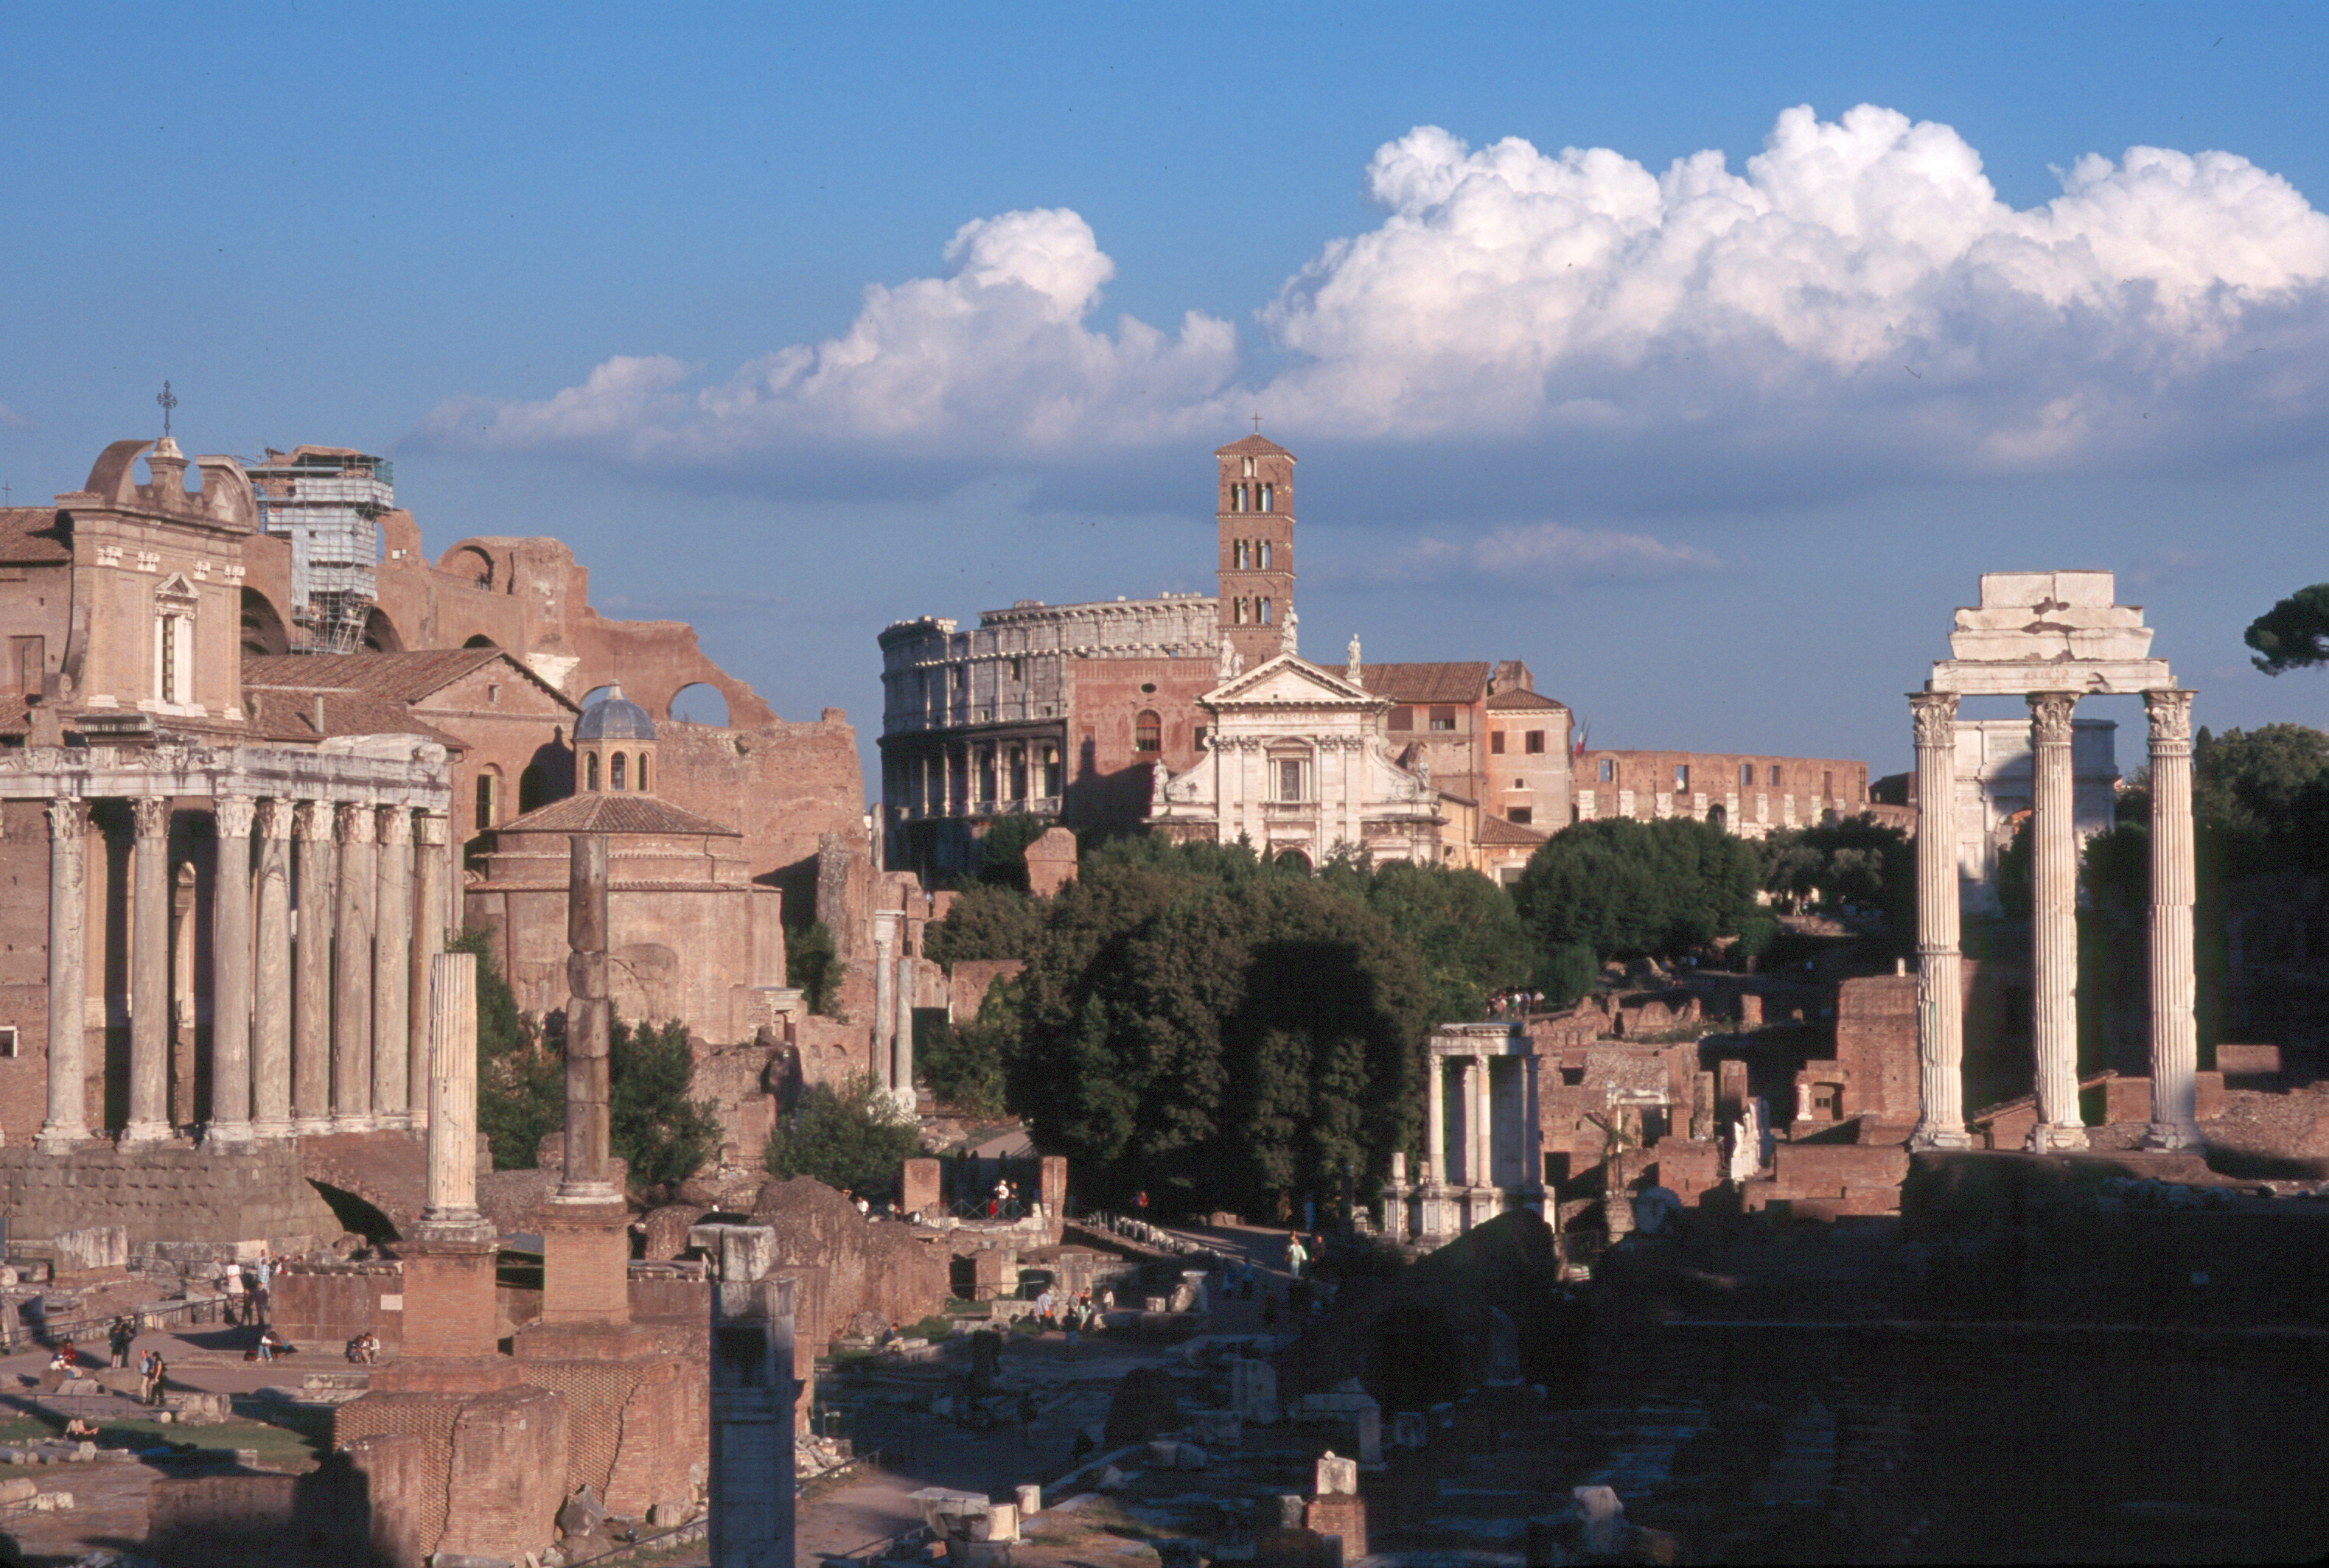
\includegraphics[width=\linewidth,height=\textheight,keepaspectratio,bb= 0 0 95 64]{/home/mkg/Dropbox/images/Scan7.jpg}
\clearpage
\onecolumn
\noindent 
\begin{lstlisting}
Filename: 2004-04-13-b_010.jpg

Date: 2002:01:01 00:00:00
Make: Minolta Co., Ltd.
Model: DiMAGE F100
Focal length (35mm eq): 90
Exposure: 0.004
F stop: 6.7
ISO: 100
Width: 2272
Height: 1704
\end{lstlisting}
\clearpage

\includegraphics[width=\linewidth,height=\textheight,keepaspectratio,bb= 0 0 2272 1704]{/home/mkg/Dropbox/images/2004-04-13-b_010.jpg}
\clearpage
\onecolumn
\noindent 
\begin{lstlisting}
Filename: 2004-12-18a_023.jpg

Date: 2004:12:18 18:59:05
Make: OLYMPUS CORPORATION
Model: C8080WZ
Exposure: 0.5
F stop: 2.5
ISO: 200
Width: 3264
Height: 2448
\end{lstlisting}
\clearpage

\includegraphics[width=\linewidth,height=\textheight,keepaspectratio,bb= 0 0 3264 2448]{/home/mkg/Dropbox/images/2004-12-18a_023.jpg}
\clearpage
\onecolumn
\noindent 
\begin{lstlisting}
Filename: 2004-12-18a_026.jpg

Date: 2004:12:18 19:00:08
Make: OLYMPUS CORPORATION
Model: C8080WZ
Exposure: 0.4
F stop: 2.5
ISO: 200
Width: 3264
Height: 2448
\end{lstlisting}
\clearpage

\includegraphics[width=\linewidth,height=\textheight,keepaspectratio,bb= 0 0 3264 2448]{/home/mkg/Dropbox/images/2004-12-18a_026.jpg}
\clearpage
\onecolumn
\noindent The only riding stable in Brooklyn.
\begin{lstlisting}
Filename: 2005-02-28a_002.jpg

Date: 2005:01:15 09:31:36
Make: OLYMPUS CORPORATION
Model: C8080WZ
Exposure: 0.008
F stop: 4.0
ISO: 50
Width: 3264
Height: 2448
\end{lstlisting}
\clearpage

\includegraphics[width=\linewidth,height=\textheight,keepaspectratio,bb= 0 0 3264 2448]{/home/mkg/Dropbox/images/2005-02-28a_002.jpg}
\clearpage
\onecolumn
\noindent 
\begin{lstlisting}
Filename: 2005-05-17a_042.jpg

Date: 2005:05:04 18:21:50
Make: OLYMPUS CORPORATION
Model: C8080WZ
Exposure: 0.016666666666666666
F stop: 3.5
ISO: 100
Width: 3264
Height: 2448
\end{lstlisting}
\clearpage

\includegraphics[width=\linewidth,height=\textheight,keepaspectratio,bb= 0 0 3264 2448]{/home/mkg/Dropbox/images/2005-05-17a_042.jpg}
\clearpage
\onecolumn
\noindent 
\begin{lstlisting}
Filename: 2005-07-09-a_100.jpg

Date: 2005:07:09 09:38:40
Make: OLYMPUS CORPORATION
Model: C8080WZ
Exposure: 0.0025
F stop: 4.0
ISO: 50
Width: 3264
Height: 2448
\end{lstlisting}
\clearpage

\includegraphics[width=\linewidth,height=\textheight,keepaspectratio,bb= 0 0 3264 2448]{/home/mkg/Dropbox/images/2005-07-09-a_100.jpg}
\clearpage
\onecolumn
\noindent 
\begin{lstlisting}
Filename: 2005-10-02-a_020.jpg

Date: 2005:08:20 11:58:52
Make: OLYMPUS CORPORATION
Model: C8080WZ
Exposure: 0.00625
F stop: 3.5
ISO: 50
Width: 3264
Height: 2448
\end{lstlisting}
\clearpage

\includegraphics[width=\linewidth,height=\textheight,keepaspectratio,bb= 0 0 3264 2448]{/home/mkg/Dropbox/images/2005-10-02-a_020.jpg}
\clearpage
\onecolumn
\noindent An old tree on our farm in Bovina, New York.
\begin{lstlisting}
Filename: 2005-10-10a_053.jpg

Date: 2005:10:10 08:58:44
Make: OLYMPUS CORPORATION
Model: C8080WZ
Exposure: 0.004
F stop: 3.5
ISO: 50
Width: 3264
Height: 2448
\end{lstlisting}
\clearpage

\includegraphics[width=\linewidth,height=\textheight,keepaspectratio,bb= 0 0 3264 2448]{/home/mkg/Dropbox/images/2005-10-10a_053.jpg}
\clearpage
\onecolumn
\noindent 
\begin{lstlisting}
Filename: 2009-08-27-a_097.jpg

Date: 2009:08:16 18:56:43
Make: Canon
Model: Canon PowerShot G7
Exposure: 0.005
F stop: 4.0
Width: 3648
Height: 2736
\end{lstlisting}
\clearpage

\includegraphics[width=\linewidth,height=\textheight,keepaspectratio,bb= 0 0 1459 1094]{/home/mkg/Dropbox/images/2009-08-27-a_097.jpg}
\clearpage
\onecolumn
\noindent 
\begin{lstlisting}
Filename: DSC01131.JPG

Date: 2013:04:01 06:21:41
Make: SONY
Model: DSC-RX100
Focal length (35mm eq): 44
Exposure: 0.01
F stop: 3.5
ISO: 125
Width: 5472
Height: 3648
\end{lstlisting}
\clearpage

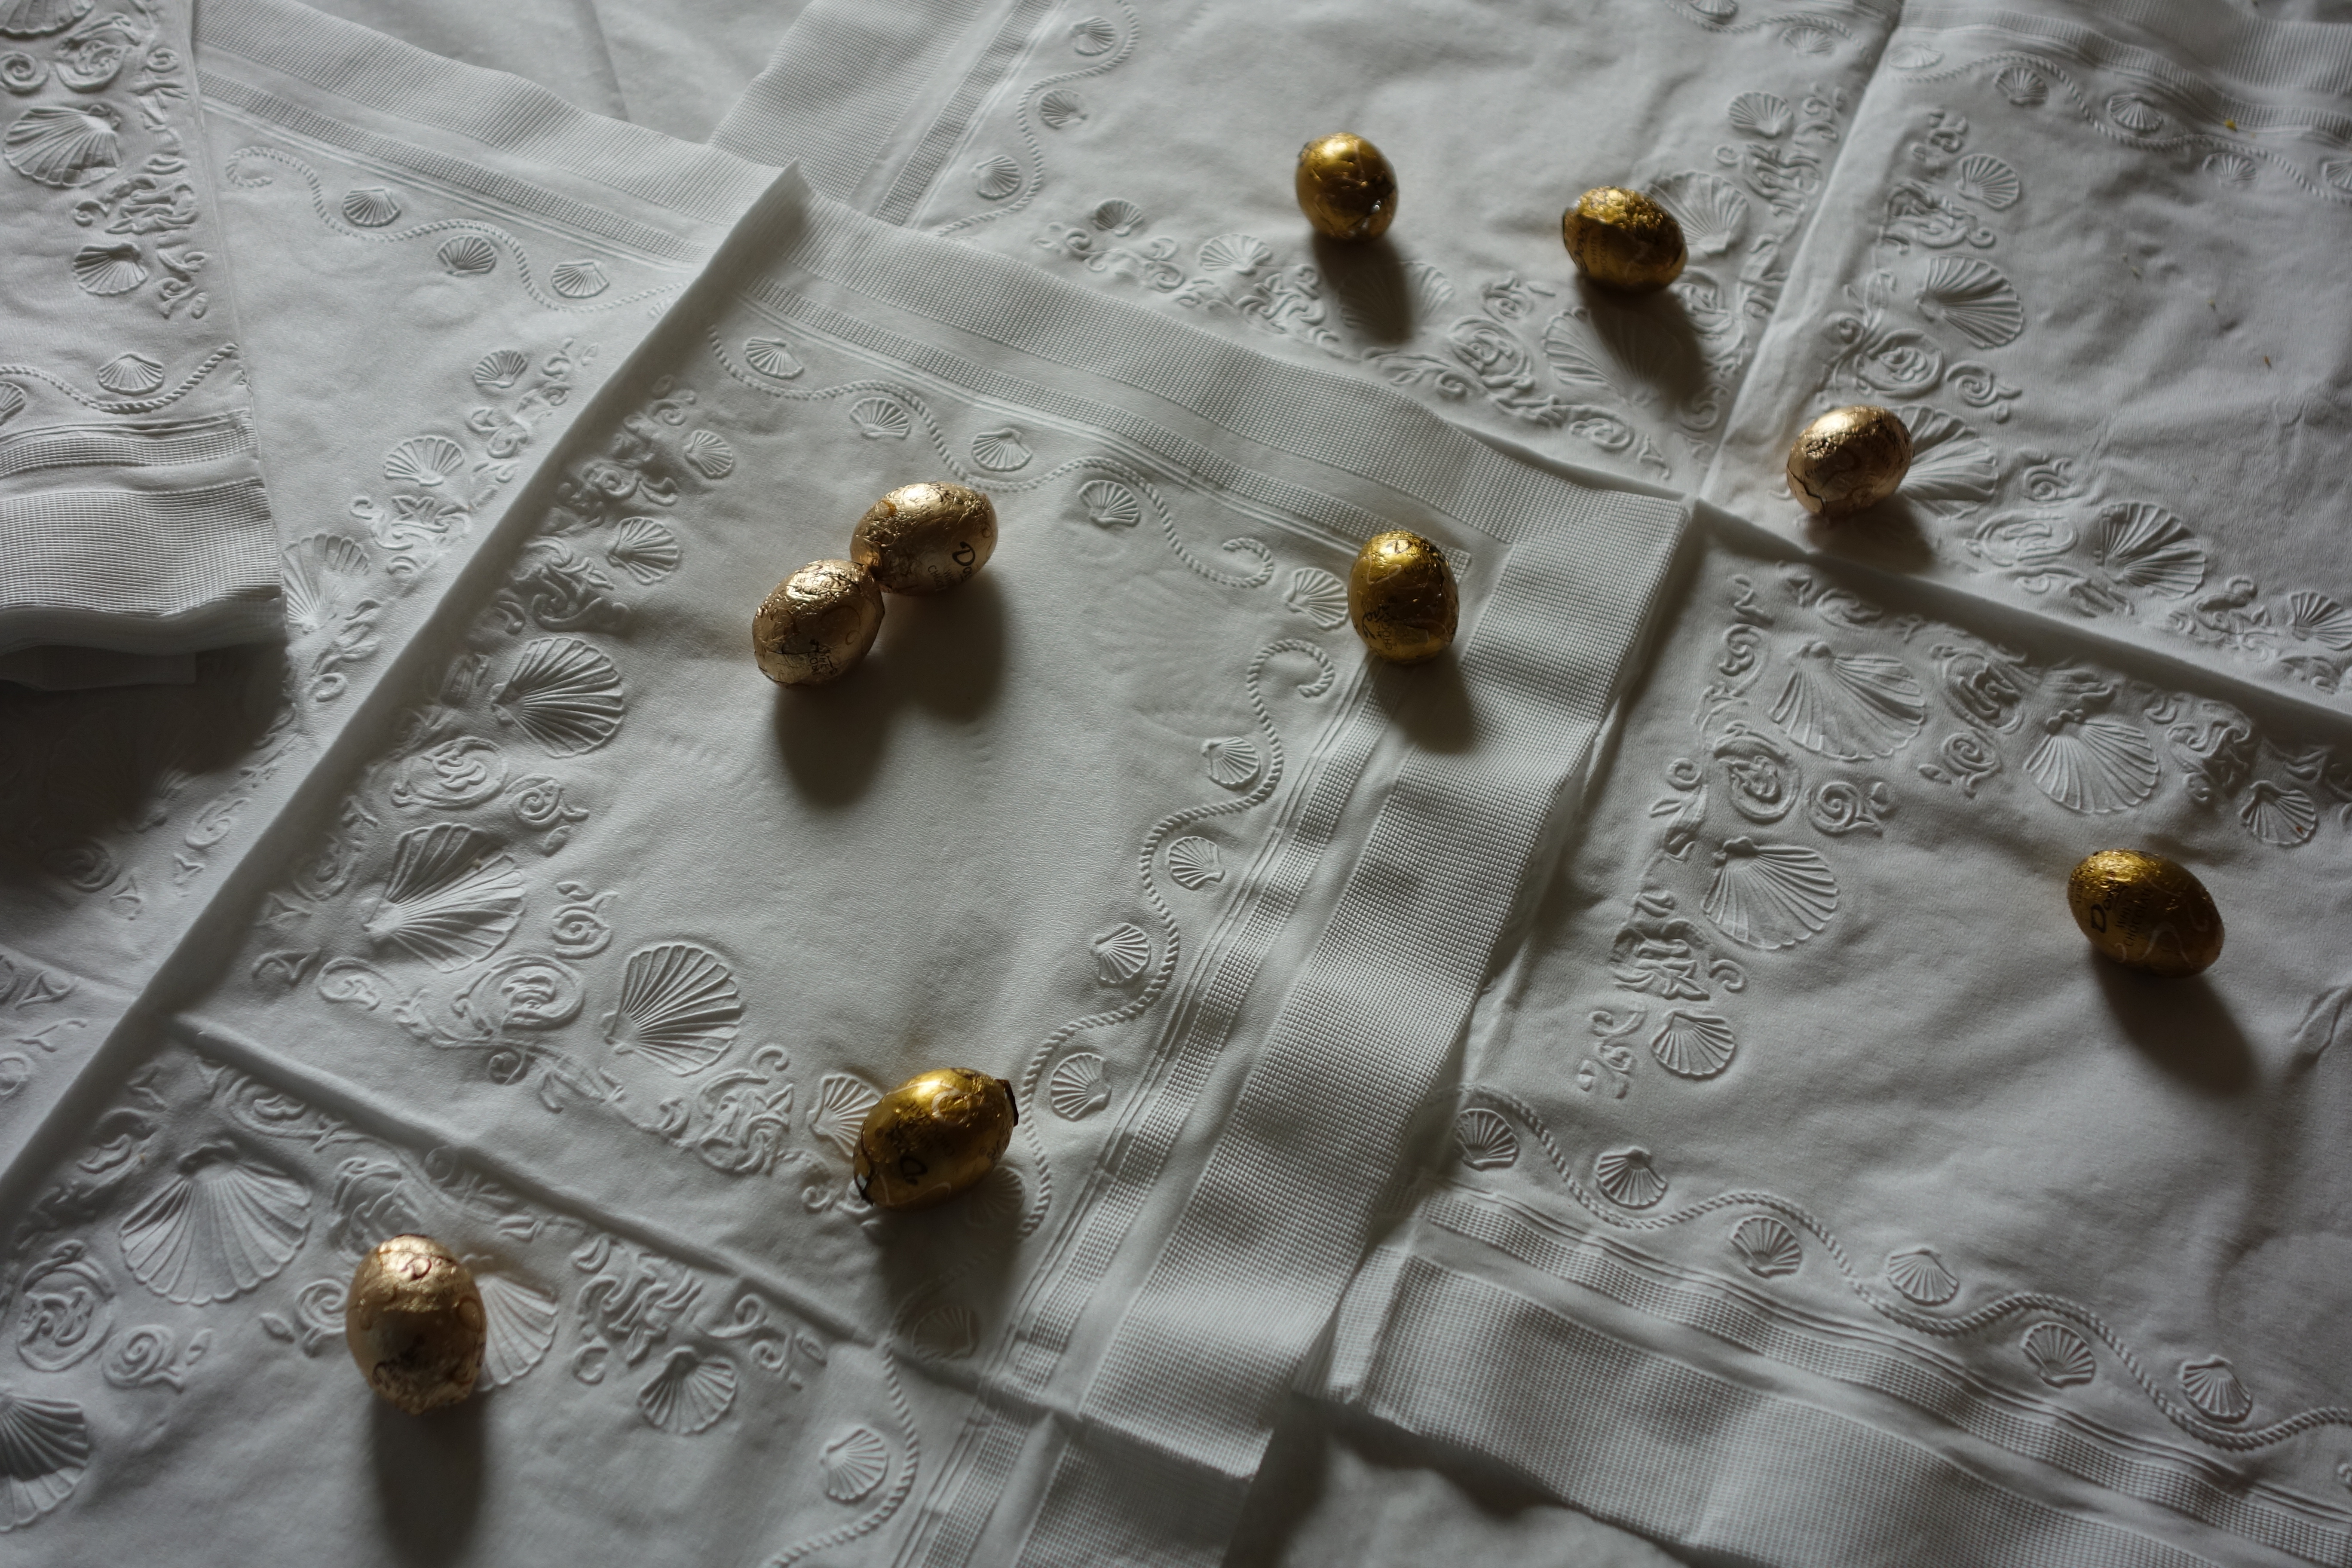
\includegraphics[width=\linewidth,height=\textheight,keepaspectratio,bb= 0 0 1126 750]{/home/mkg/Dropbox/images/DSC01131.JPG}
\clearpage
\onecolumn
\noindent 
\begin{lstlisting}
Filename: DSC01240.JPG

Date: 2013:04:06 18:06:00
Make: SONY
Model: DSC-RX100
Focal length (35mm eq): 54
Exposure: 0.01
F stop: 4.5
ISO: 125
Width: 5472
Height: 3648
\end{lstlisting}
\clearpage

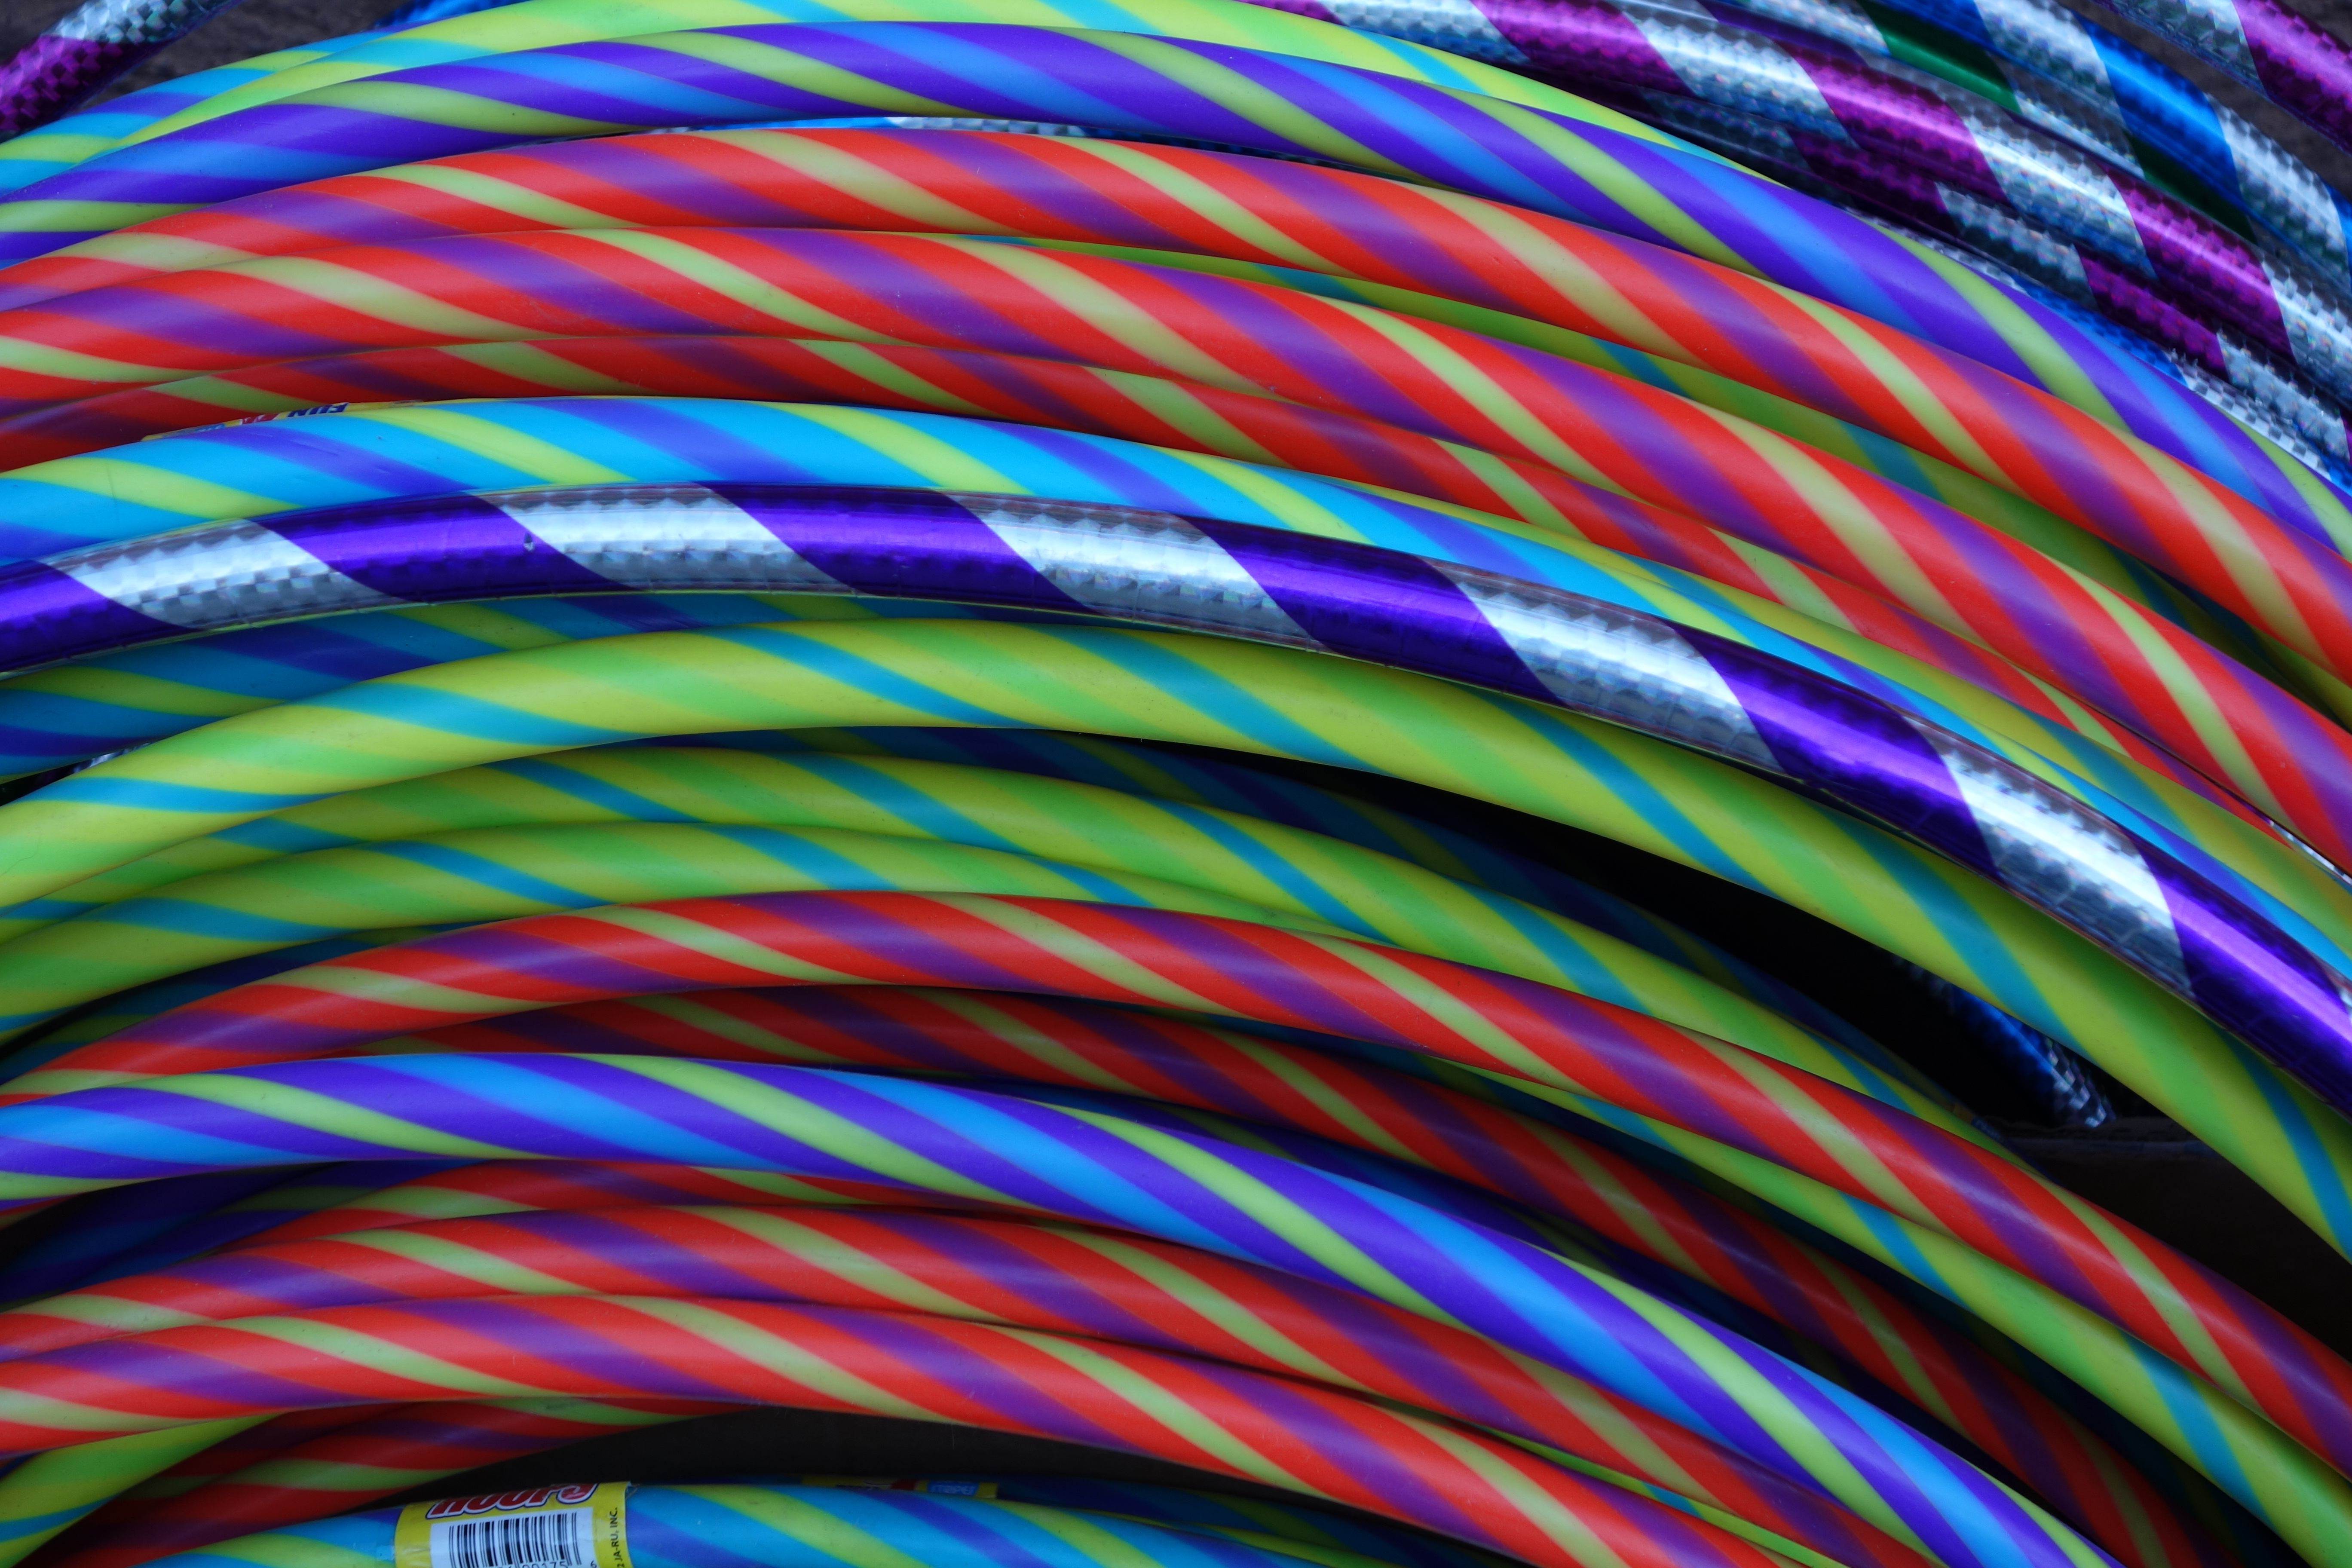
\includegraphics[width=\linewidth,height=\textheight,keepaspectratio,bb= 0 0 1126 750]{/home/mkg/Dropbox/images/DSC01240.JPG}
\clearpage
\onecolumn
\noindent The old ice cream stand in Stamford, New York. Replaced by a newer (but not quite as friendly and funky) version.
\begin{lstlisting}
Filename: DSC01577.JPG

Date: 2013:08:25 19:38:23
Make: SONY
Model: DSC-RX100
Focal length (35mm eq): 100
Exposure: 0.01
F stop: 4.9
ISO: 800
Width: 5472
Height: 3648
\end{lstlisting}
\clearpage

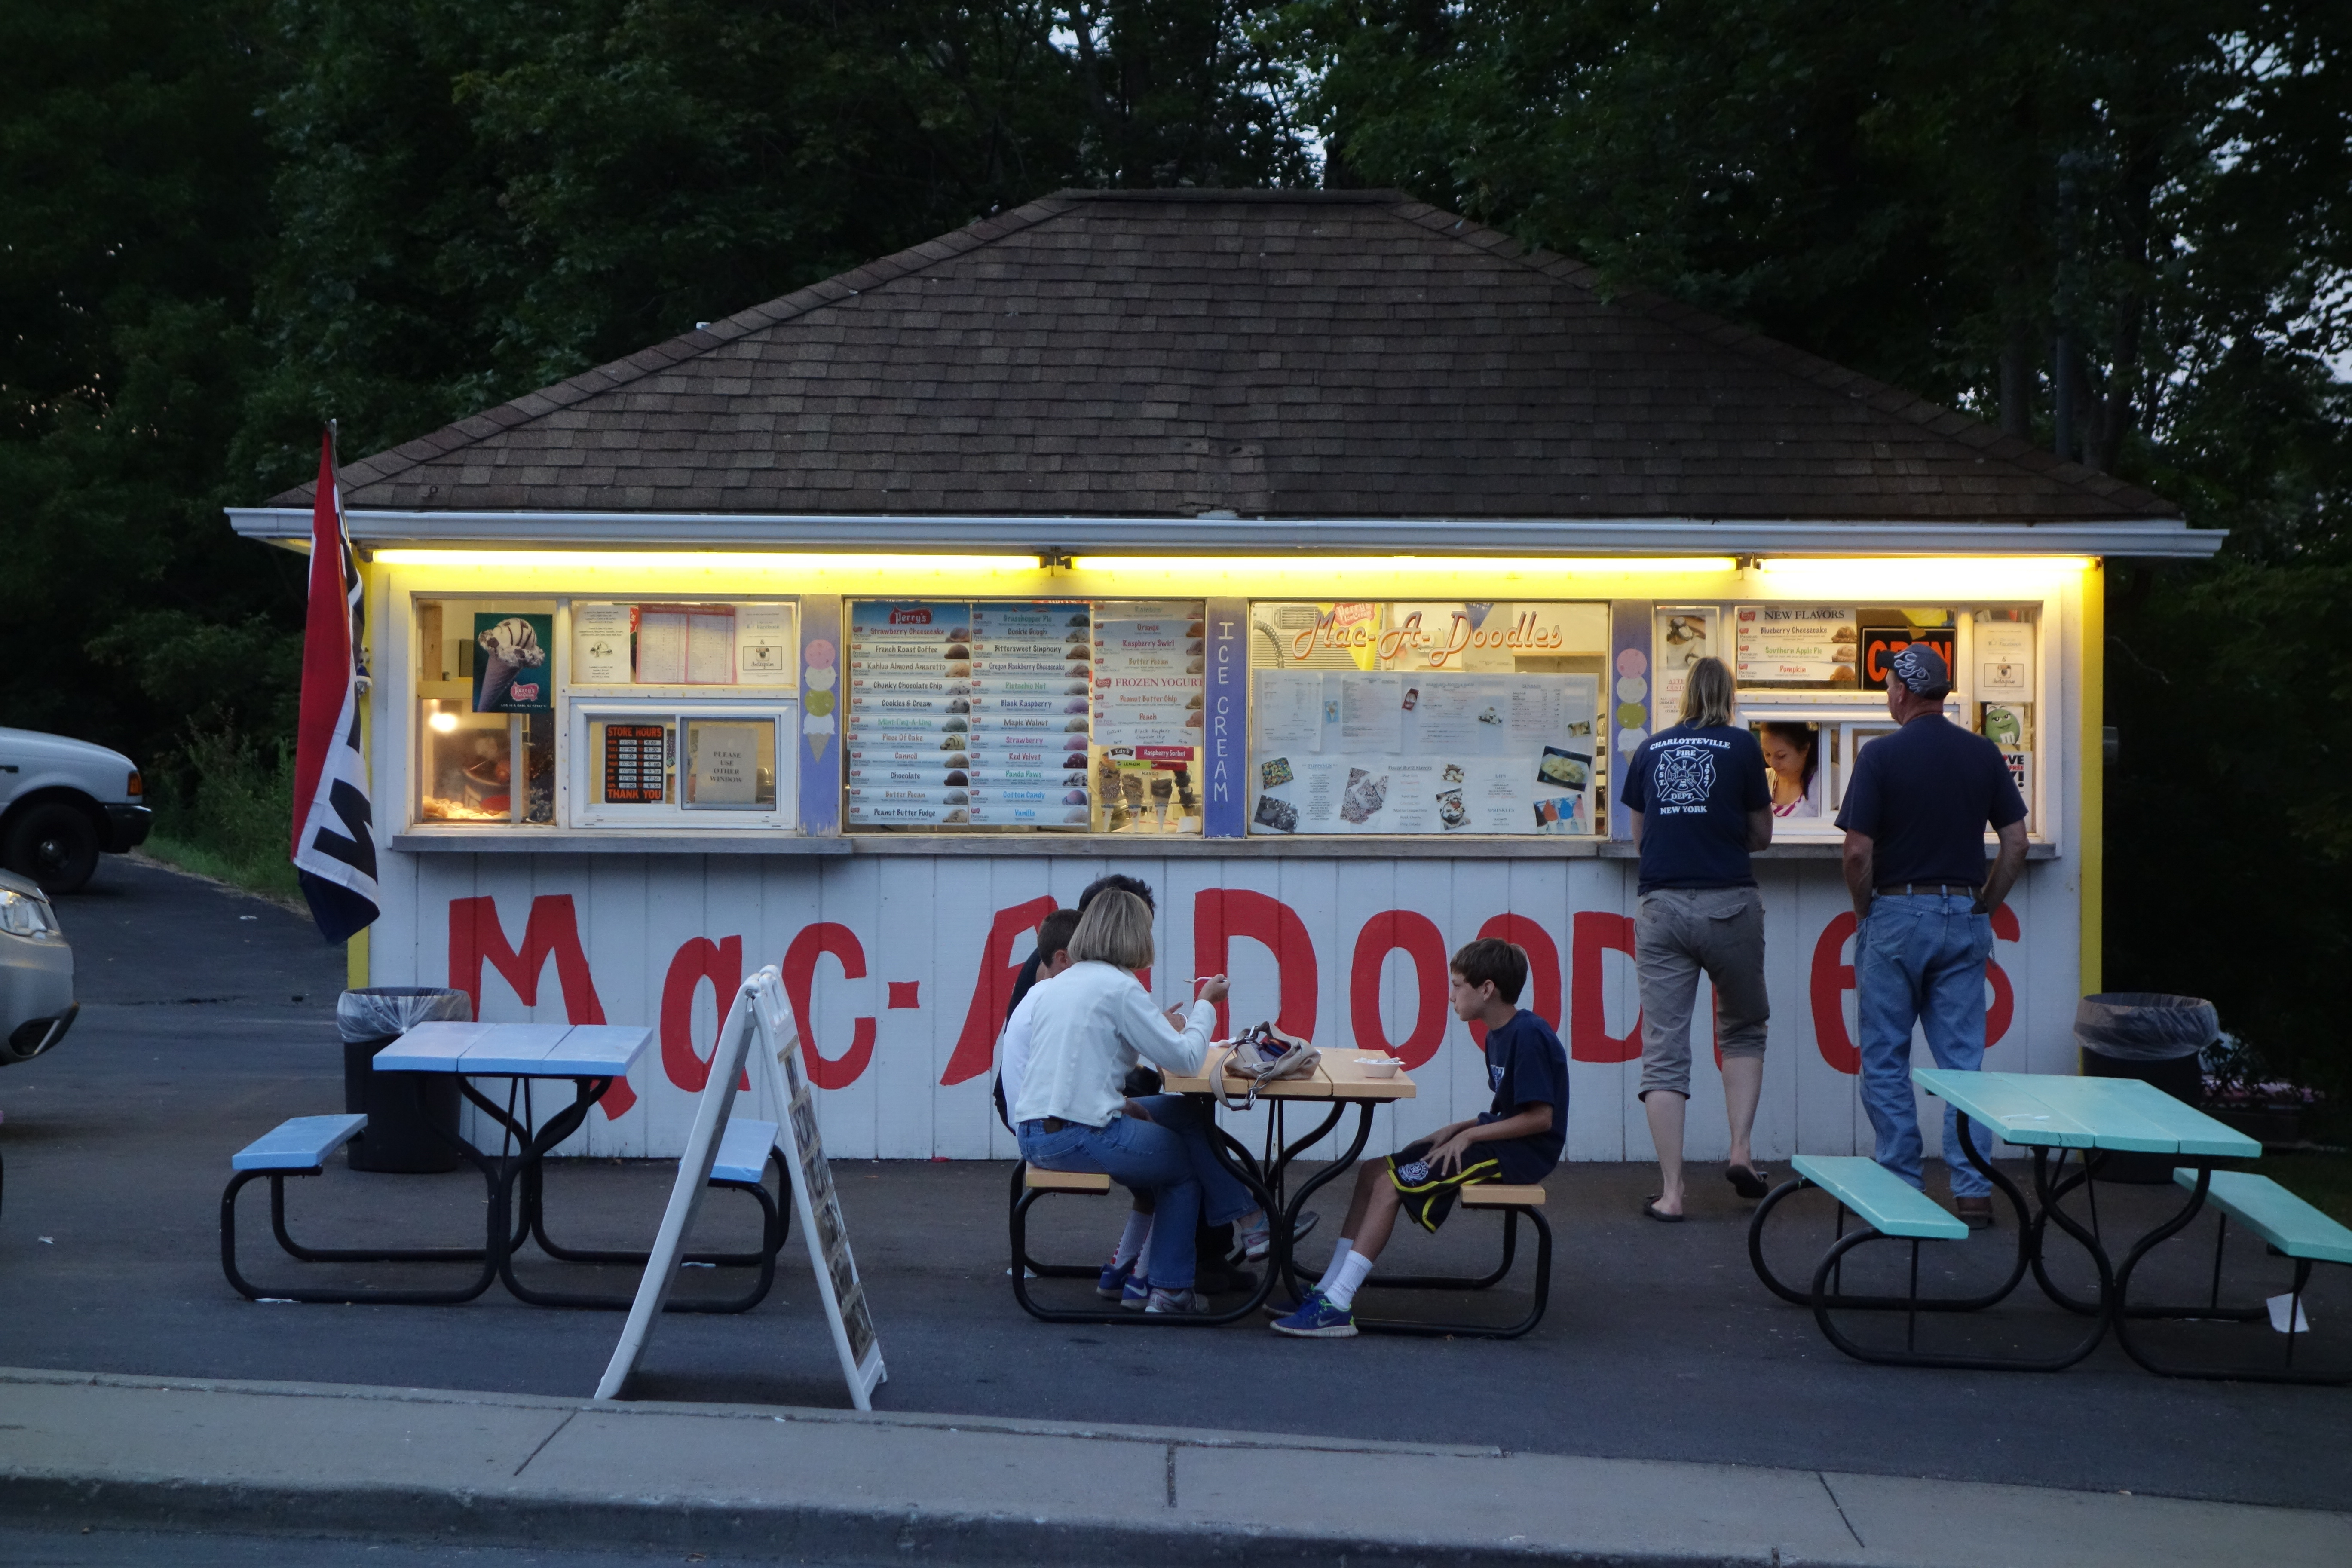
\includegraphics[width=\linewidth,height=\textheight,keepaspectratio,bb= 0 0 1126 750]{/home/mkg/Dropbox/images/DSC01577.JPG}
\clearpage
\onecolumn
\noindent Computer music luminaries Richard Boulanger (left) and Jean-Claude Risset, and their spouses, at the 2nd International Csound Conference, Berklee School of Music, Boston.
\begin{lstlisting}
Filename: DSC01723.JPG

Date: 2013:10:25 10:07:59
Make: SONY
Model: DSC-RX100
Focal length (35mm eq): 46
Exposure: 0.02
F stop: 3.2
ISO: 3200
Width: 5368
Height: 3484
\end{lstlisting}
\clearpage

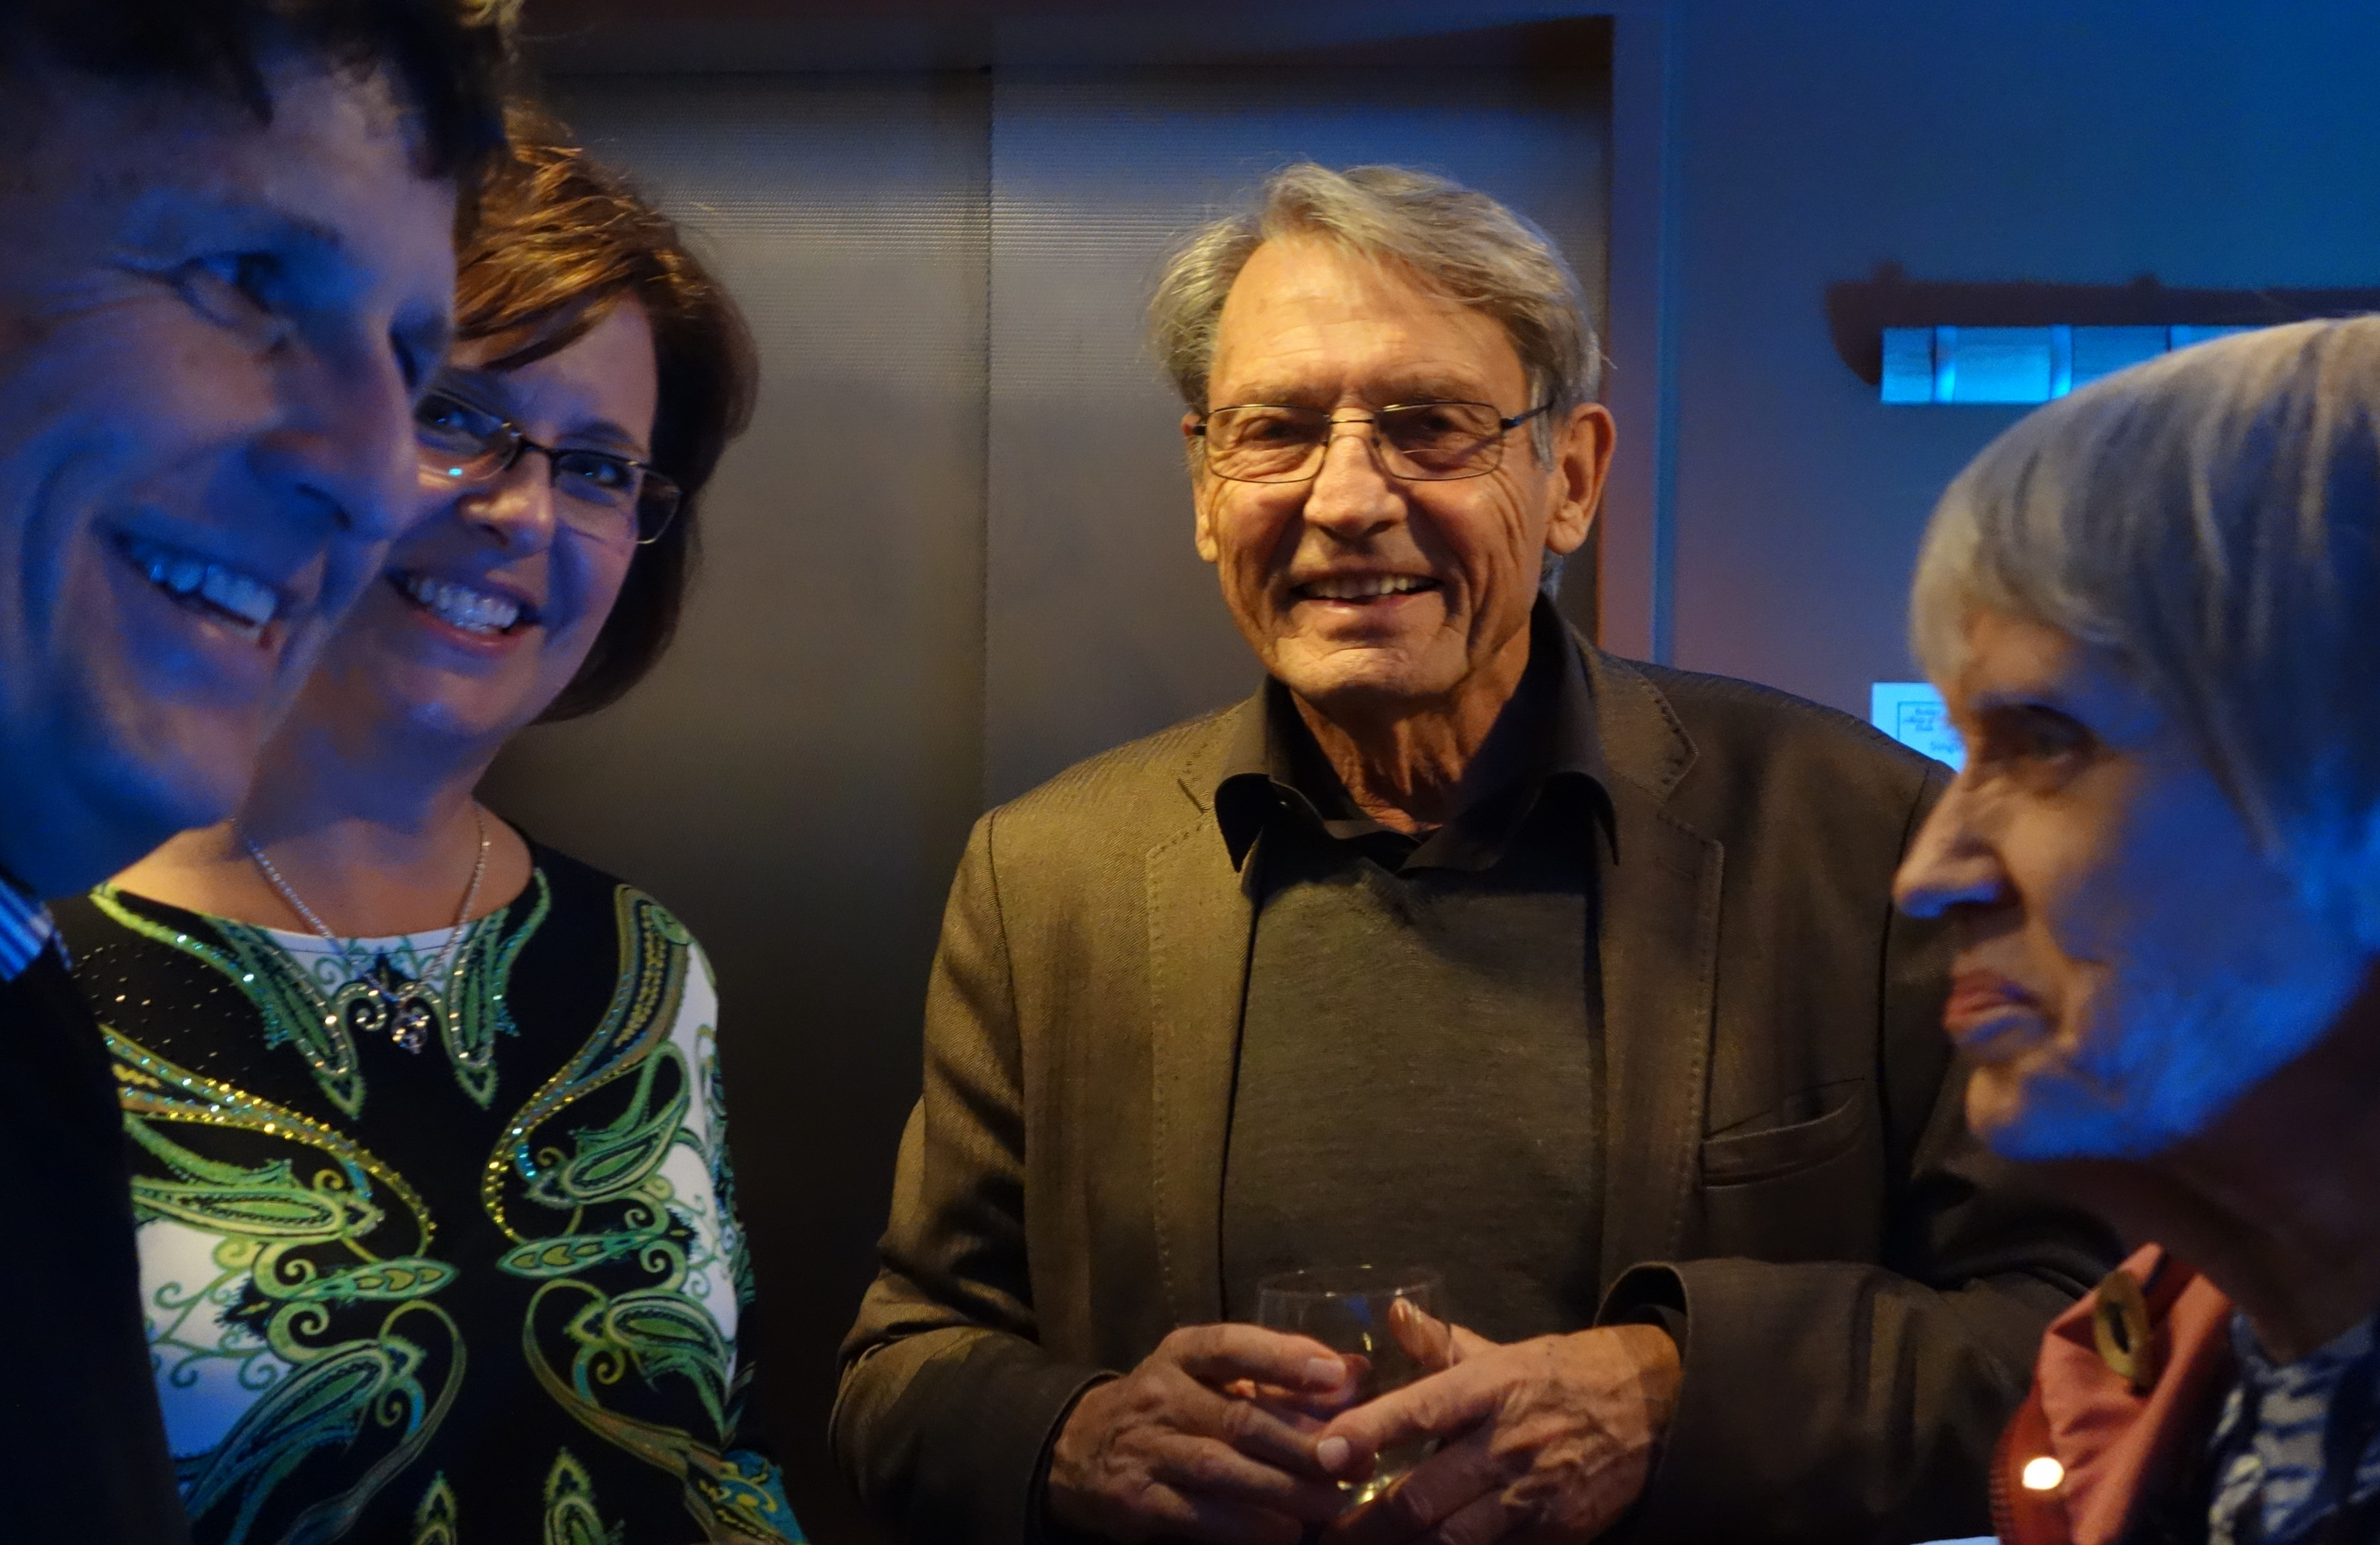
\includegraphics[width=\linewidth,height=\textheight,keepaspectratio,bb= 0 0 1104 717]{/home/mkg/Dropbox/images/DSC01723.JPG}
\clearpage
\onecolumn
\noindent Magazine covers, Girona, Spain.
\begin{lstlisting}
Filename: DSC02503.JPG

Date: 2013:12:06 07:04:13
Make: SONY
Model: DSC-RX100
Focal length (35mm eq): 78
Exposure: 0.002
F stop: 5.6
ISO: 125
Width: 5472
Height: 3648
\end{lstlisting}
\clearpage

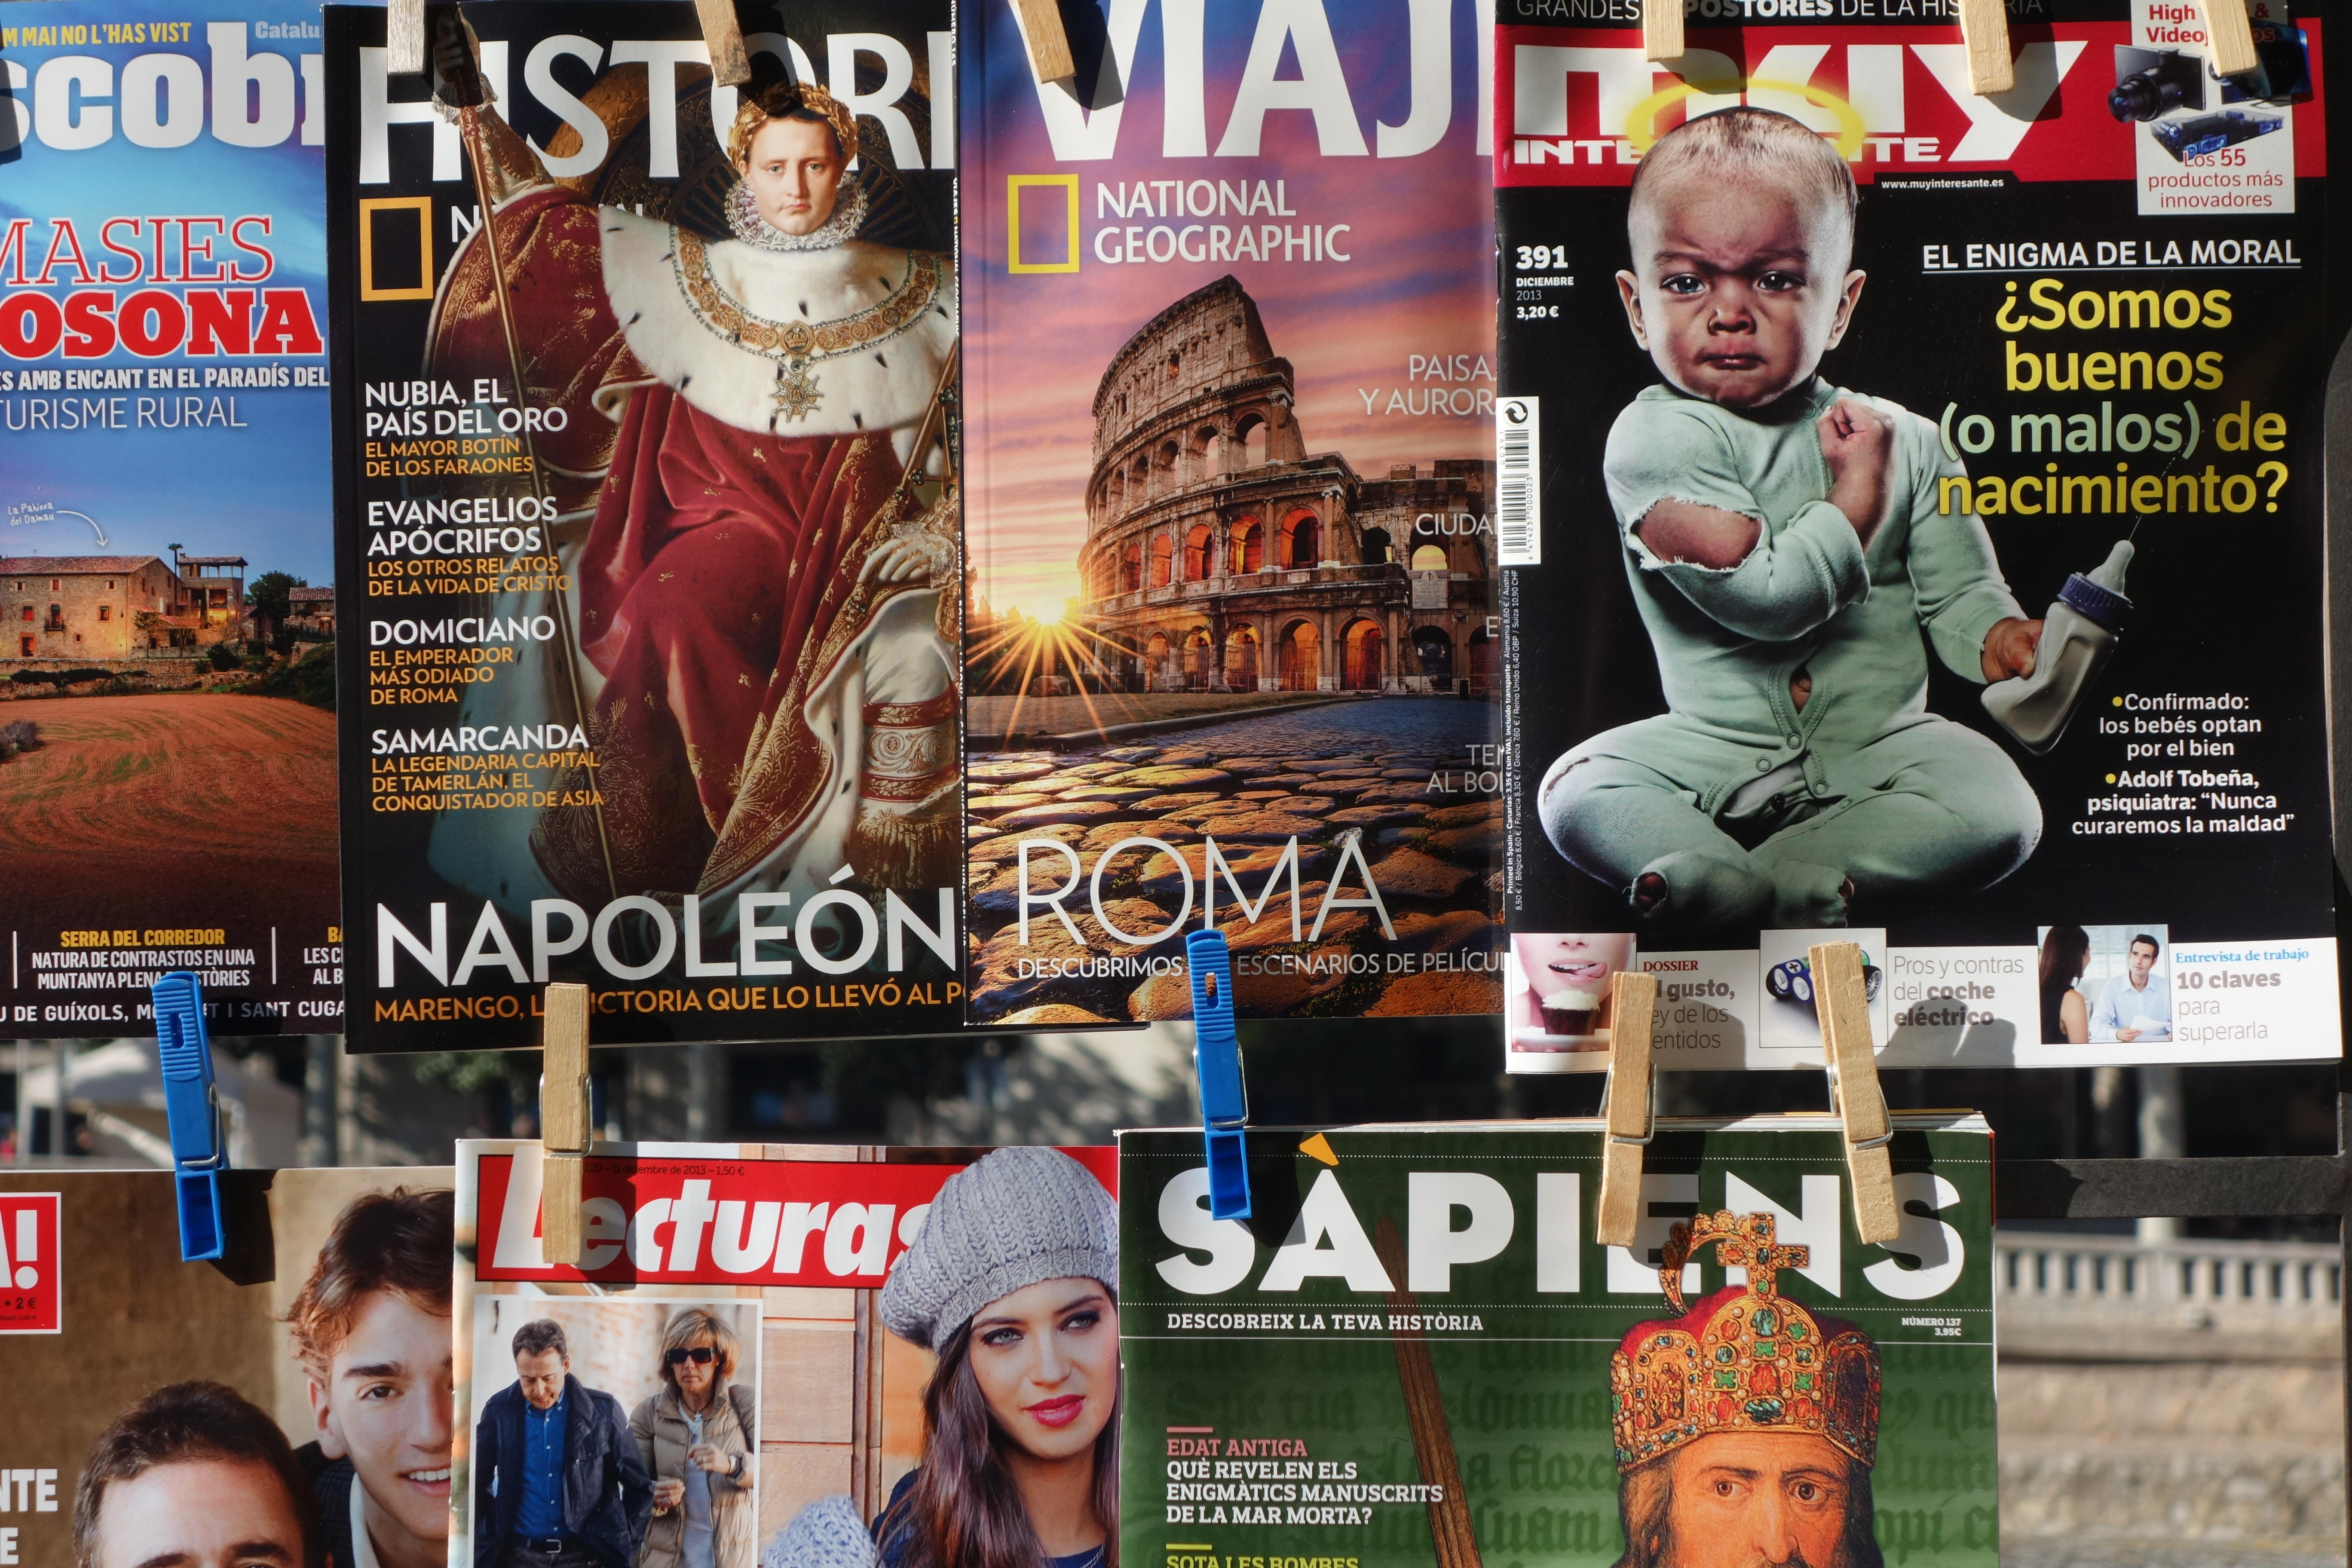
\includegraphics[width=\linewidth,height=\textheight,keepaspectratio,bb= 0 0 1126 750]{/home/mkg/Dropbox/images/DSC02503.JPG}
\clearpage
\onecolumn
\noindent 
\begin{lstlisting}
Filename: DSC02654.JPG

Date: 2013:12:08 09:24:07
Make: SONY
Model: DSC-RX100
Focal length (35mm eq): 100
Exposure: 0.005
F stop: 5.6
ISO: 125
Width: 5472
Height: 3648
\end{lstlisting}
\clearpage

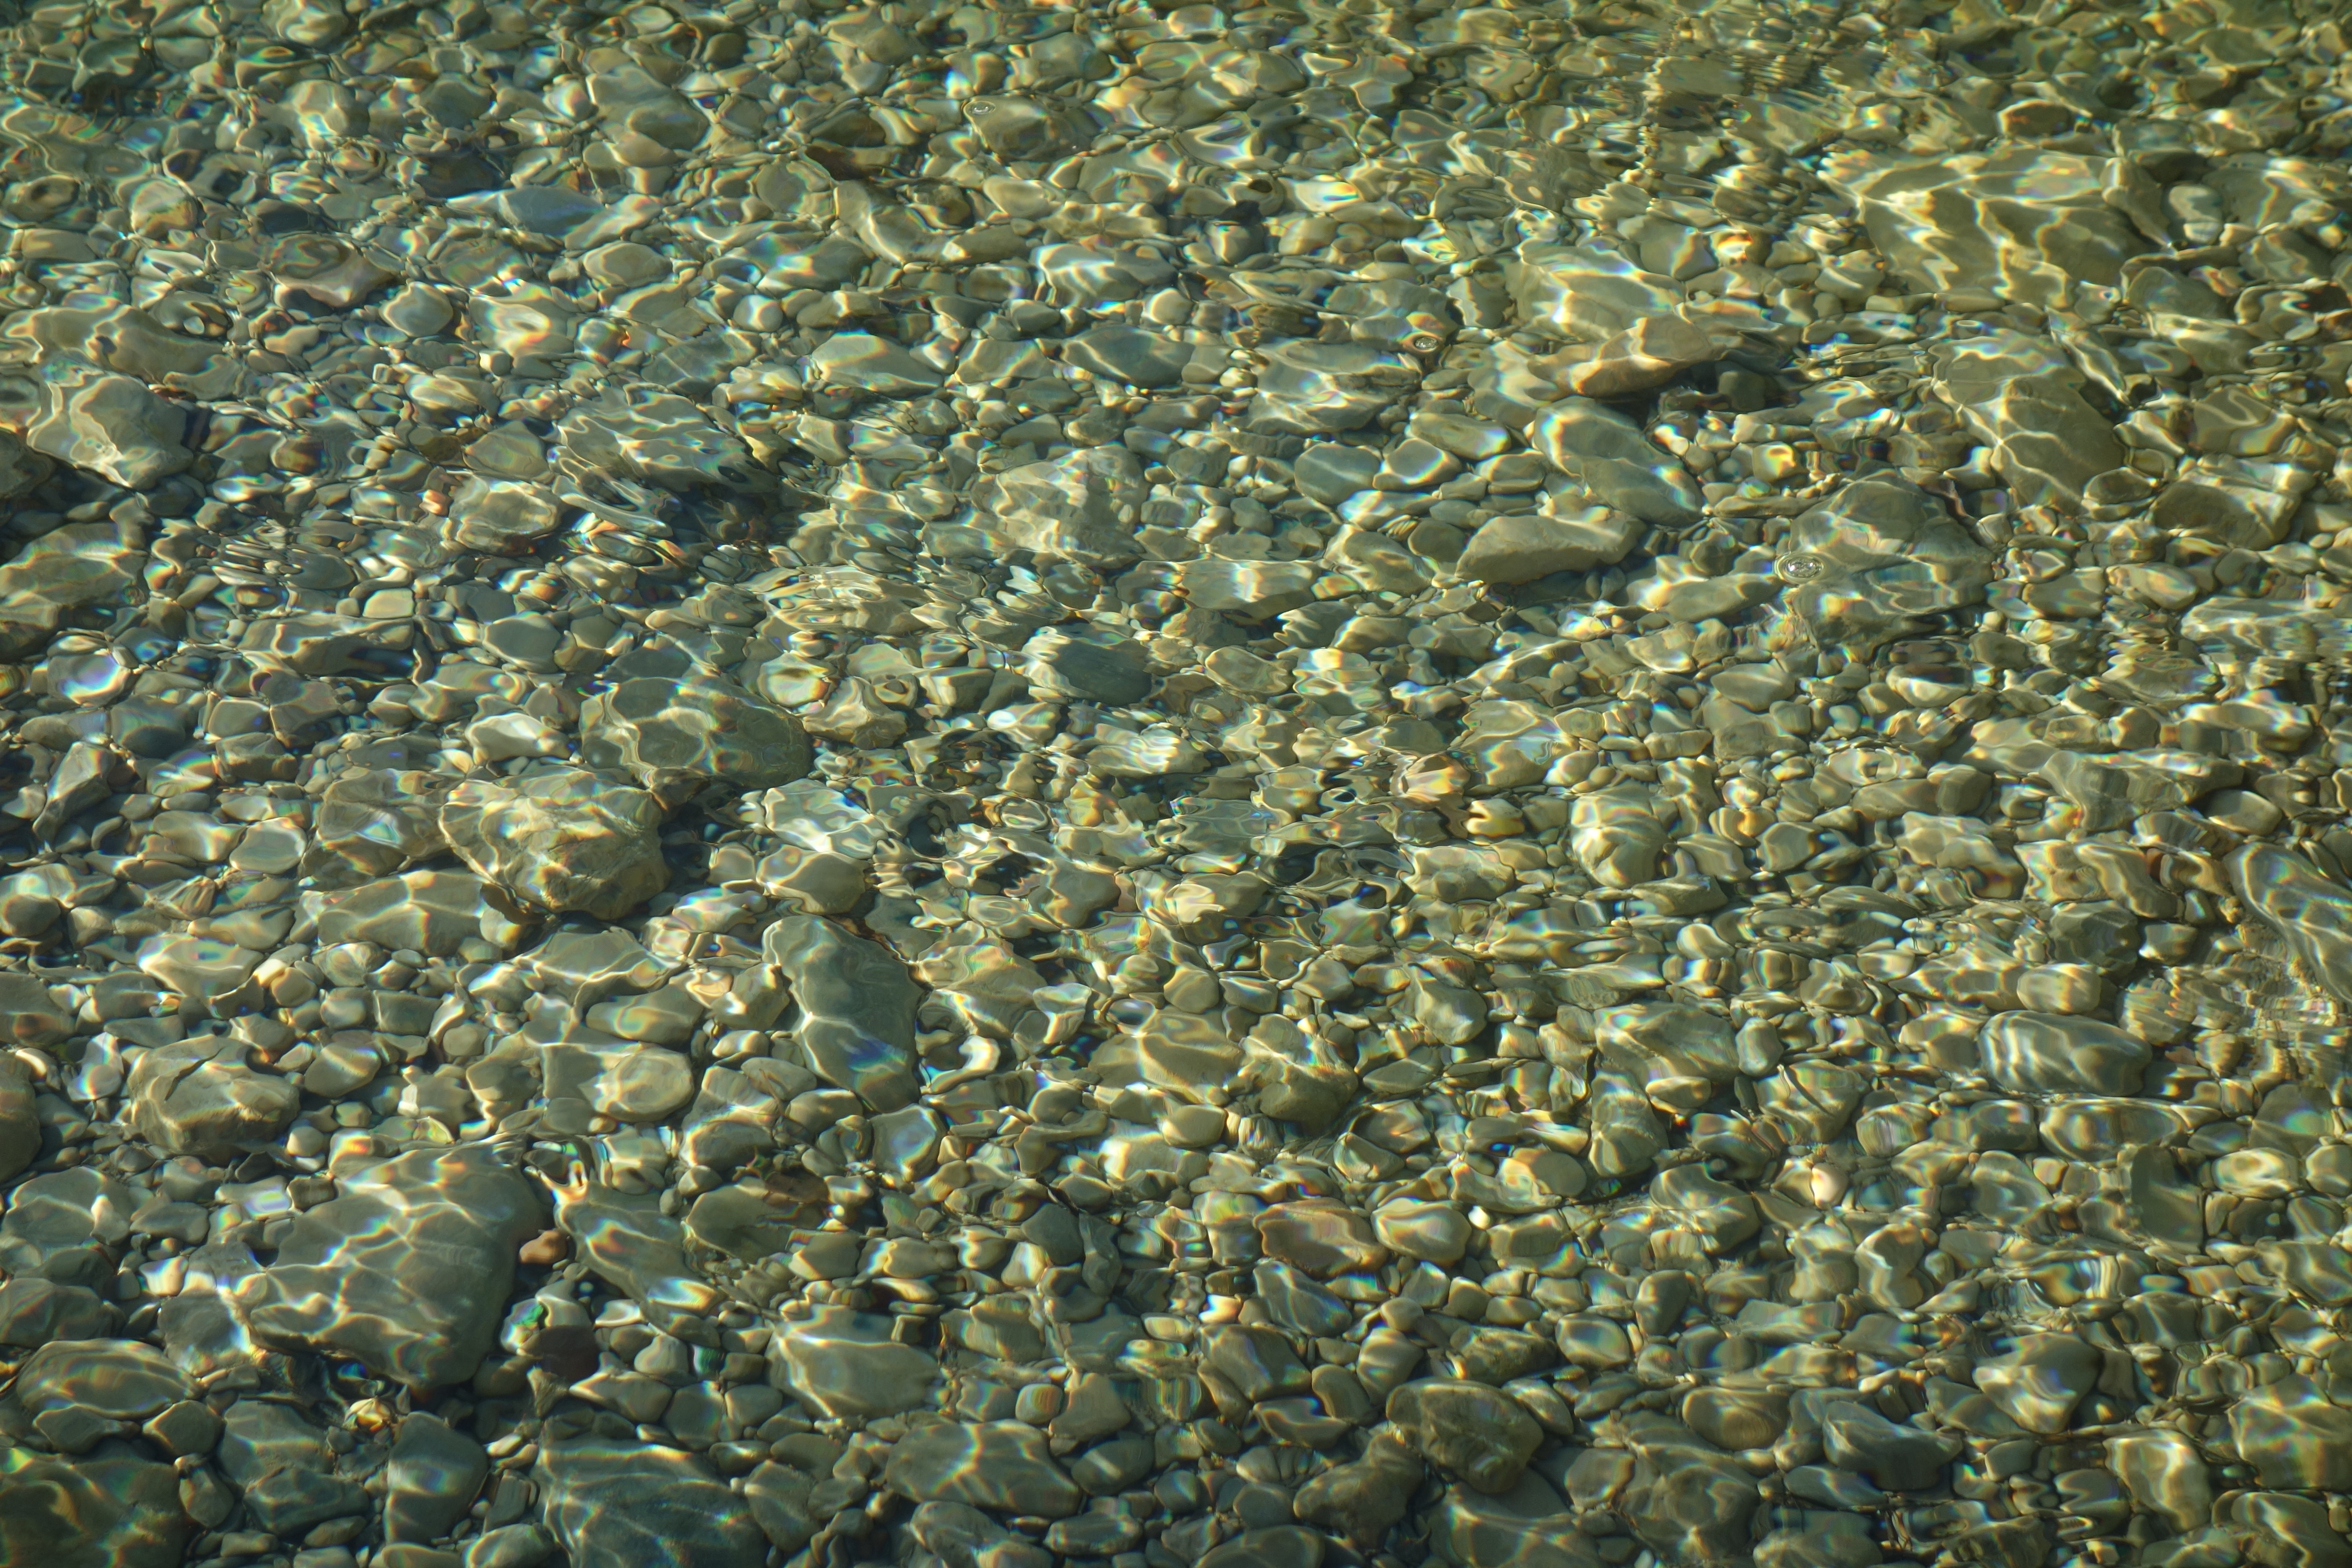
\includegraphics[width=\linewidth,height=\textheight,keepaspectratio,bb= 0 0 1126 750]{/home/mkg/Dropbox/images/DSC02654.JPG}
\clearpage
\onecolumn
\noindent 
\begin{lstlisting}
Filename: RX100M5/100MSDCF/DSC06075.JPG

Date: 2019:03:09 22:01:42
Make: SONY
Model: DSC-RX100M5
Focal length (35mm eq): 70
Exposure: 0.0125
F stop: 5.6
ISO: 125
Width: 5472
Height: 3648
\end{lstlisting}
\clearpage

\includegraphics[width=\linewidth,height=\textheight,keepaspectratio,bb= 0 0 1126 750]{/home/mkg/Dropbox/images/RX100M5/100MSDCF/DSC06075.JPG}
\clearpage
\onecolumn
\noindent 
\begin{lstlisting}
Filename: RX100/100MSDCF/DSC06643.JPG

Date: 2019:03:29 15:46:37
Make: SONY
Model: DSC-RX100M5
Focal length (35mm eq): 24
Exposure: 0.00625
F stop: 4.0
ISO: 125
Width: 5472
Height: 3648
\end{lstlisting}
\clearpage

\includegraphics[width=\linewidth,height=\textheight,keepaspectratio,bb= 0 0 1126 750]{/home/mkg/Dropbox/images/RX100/100MSDCF/DSC06643.JPG}
\clearpage
\onecolumn
\noindent Chinese Garden, Dunedin, New Zealand.
\begin{lstlisting}
Filename: RX100M5/100MSDCF/DSC06552.JPG

Date: 2019:03:26 22:40:10
Make: SONY
Model: DSC-RX100M5
Focal length (35mm eq): 70
Exposure: 0.0015625
F stop: 4.0
ISO: 125
Width: 5472
Height: 3648
\end{lstlisting}
\clearpage

\includegraphics[width=\linewidth,height=\textheight,keepaspectratio,bb= 0 0 1126 750]{/home/mkg/Dropbox/images/RX100M5/100MSDCF/DSC06552.JPG}
\clearpage
\onecolumn
\noindent Lower East Side, Manhattan.
\begin{lstlisting}
Filename: RX100/100MSDCF/DSC00956.JPG

Date: 2016:12:03 19:03:49
Make: SONY
Model: DSC-RX100
Focal length (35mm eq): 28
Exposure: 0.025
F stop: 1.8
ISO: 3200
Width: 5472
Height: 3648
\end{lstlisting}
\clearpage

\includegraphics[width=\linewidth,height=\textheight,keepaspectratio,bb= 0 0 1126 750]{/home/mkg/Dropbox/images/RX100/100MSDCF/DSC00956.JPG}
\clearpage
\onecolumn
\noindent The Father offering the Son, Narbonne, France.
\begin{lstlisting}
Filename: DSC02857.JPG

Date: 2013:12:11 10:47:13
Make: SONY
Model: DSC-RX100
Focal length (35mm eq): 57
Exposure: 0.06666666666666667
F stop: 3.5
ISO: 800
Width: 3476
Height: 5362
\end{lstlisting}
\clearpage

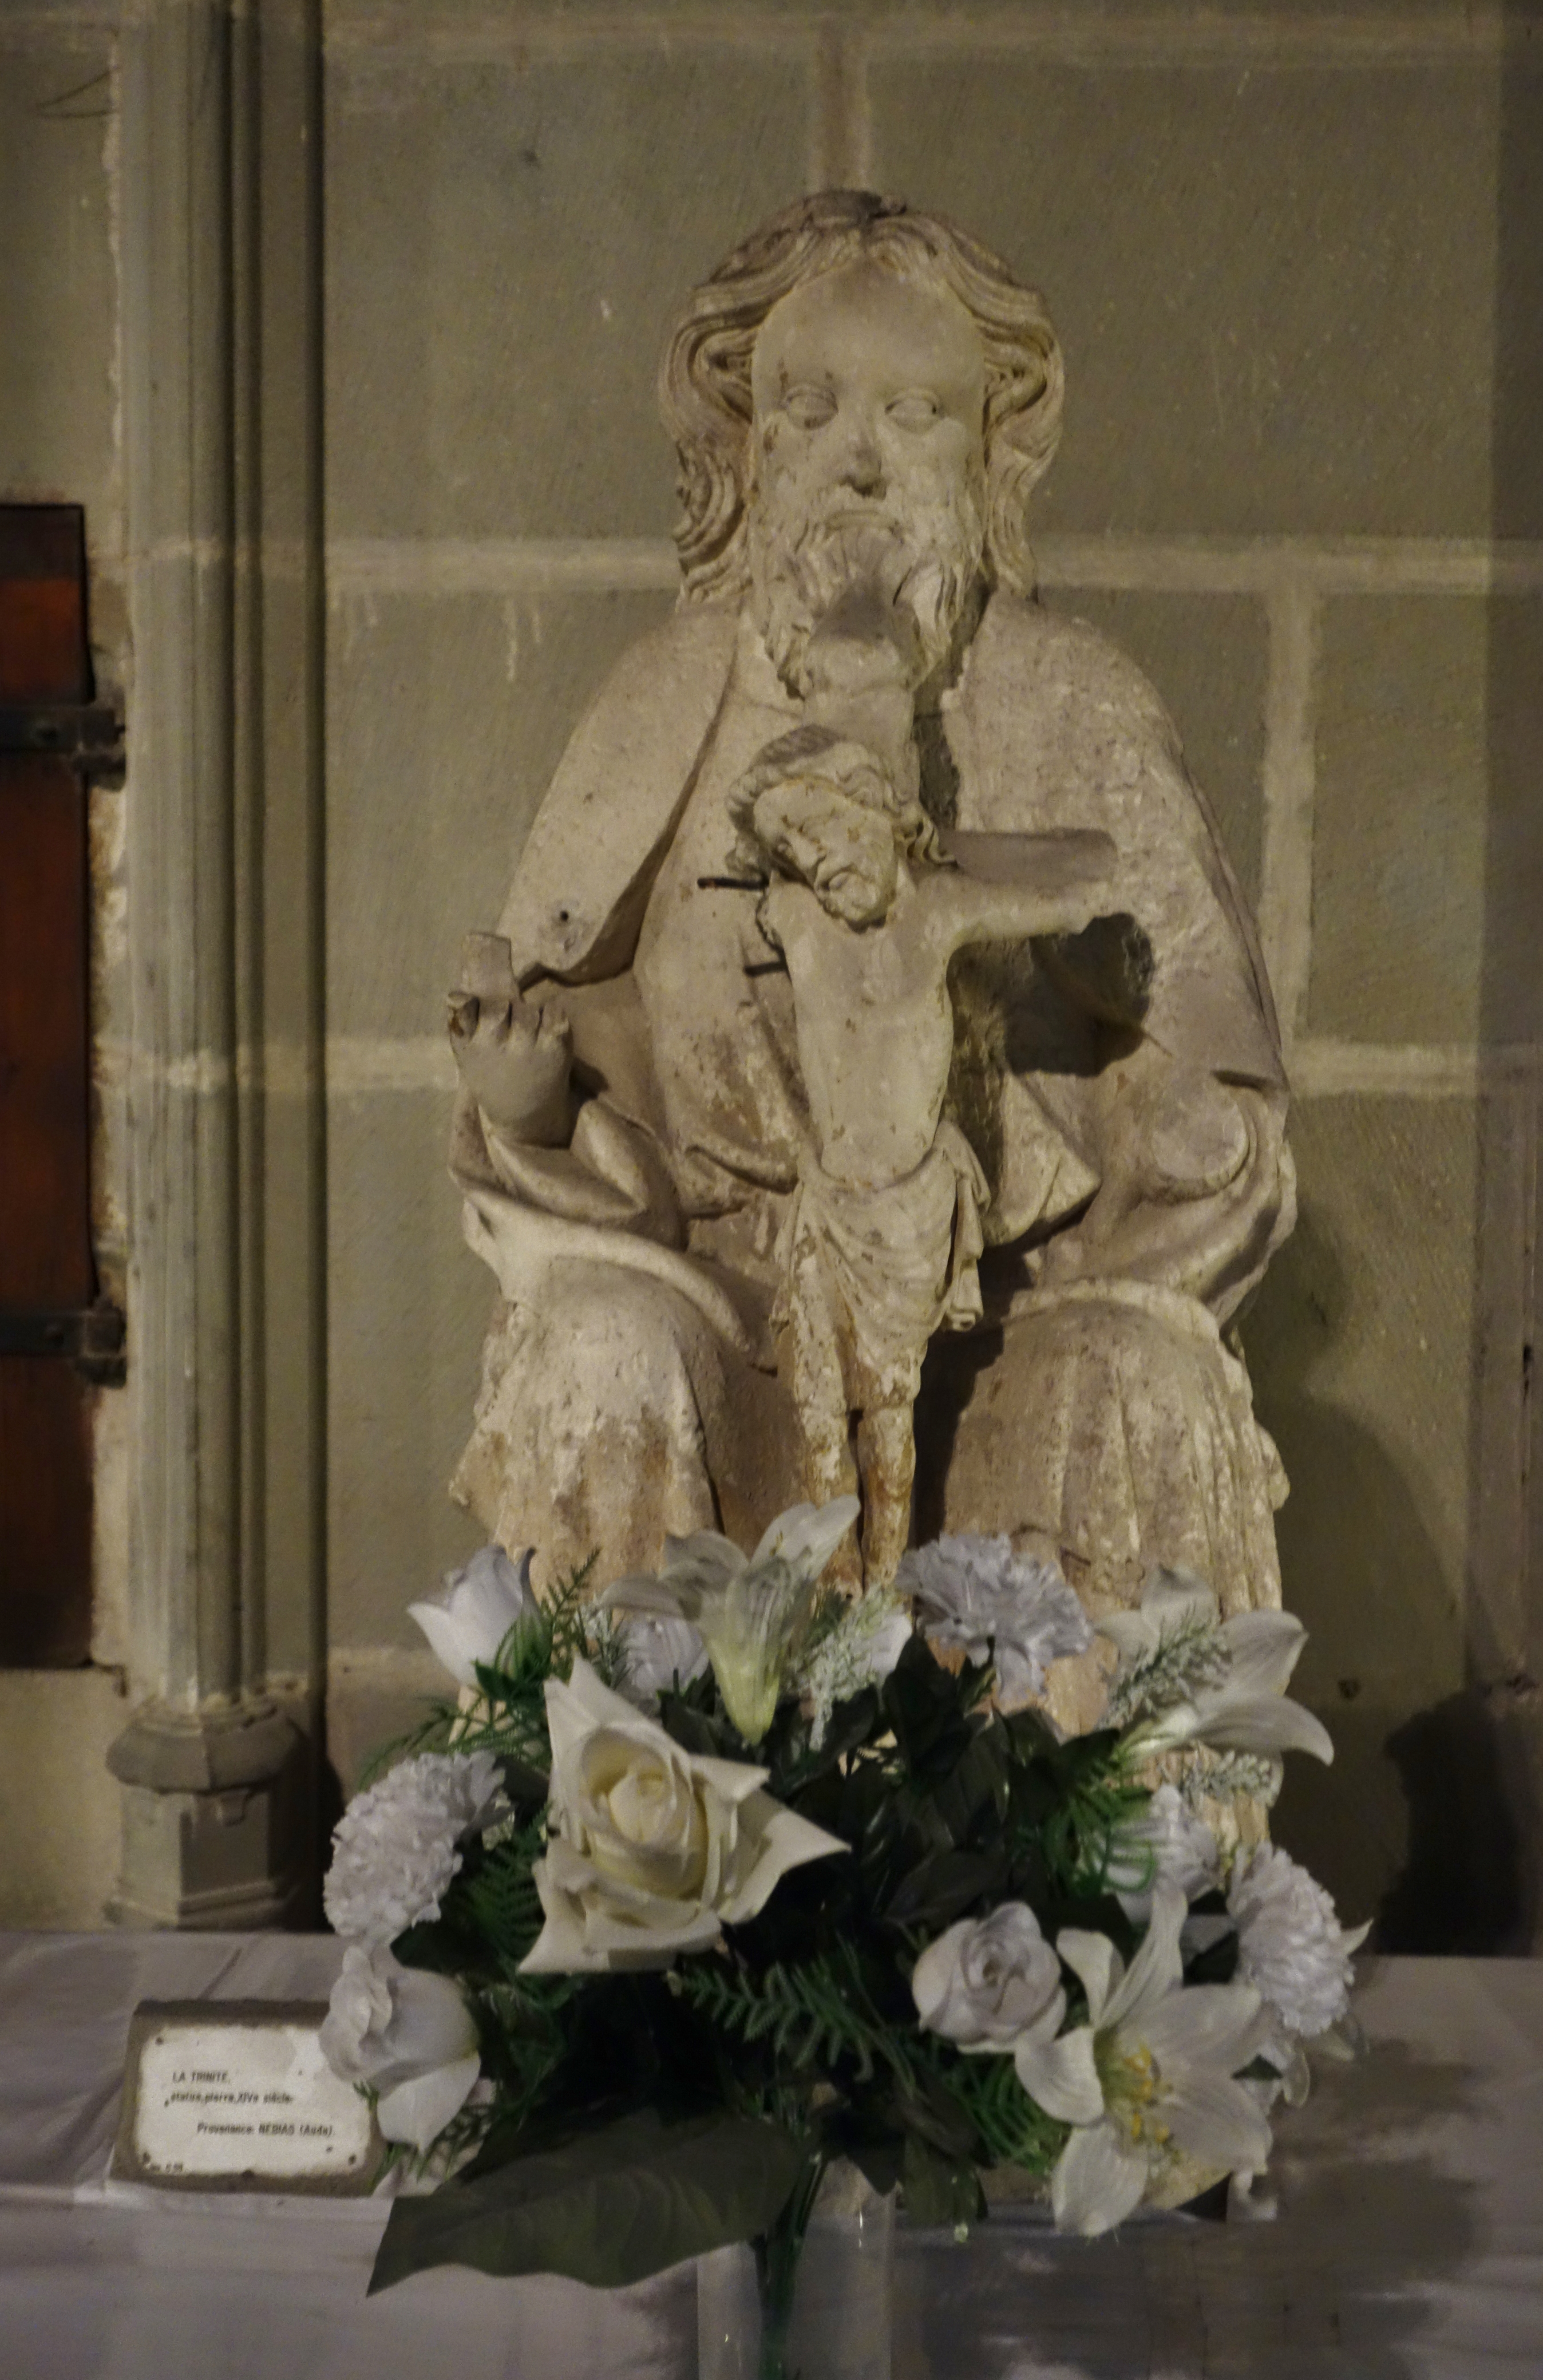
\includegraphics[width=\linewidth,height=\textheight,keepaspectratio,bb= 0 0 715 1103]{/home/mkg/Dropbox/images/DSC02857.JPG}
\clearpage
\onecolumn
\noindent Christmas carnival in Carcassone, France.
\begin{lstlisting}
Filename: DSC02910.JPG

Date: 2013:12:11 13:36:30
Make: SONY
Model: DSC-RX100
Focal length (35mm eq): 72
Exposure: 0.0125
F stop: 4.0
ISO: 3200
Width: 5376
Height: 3500
\end{lstlisting}
\clearpage

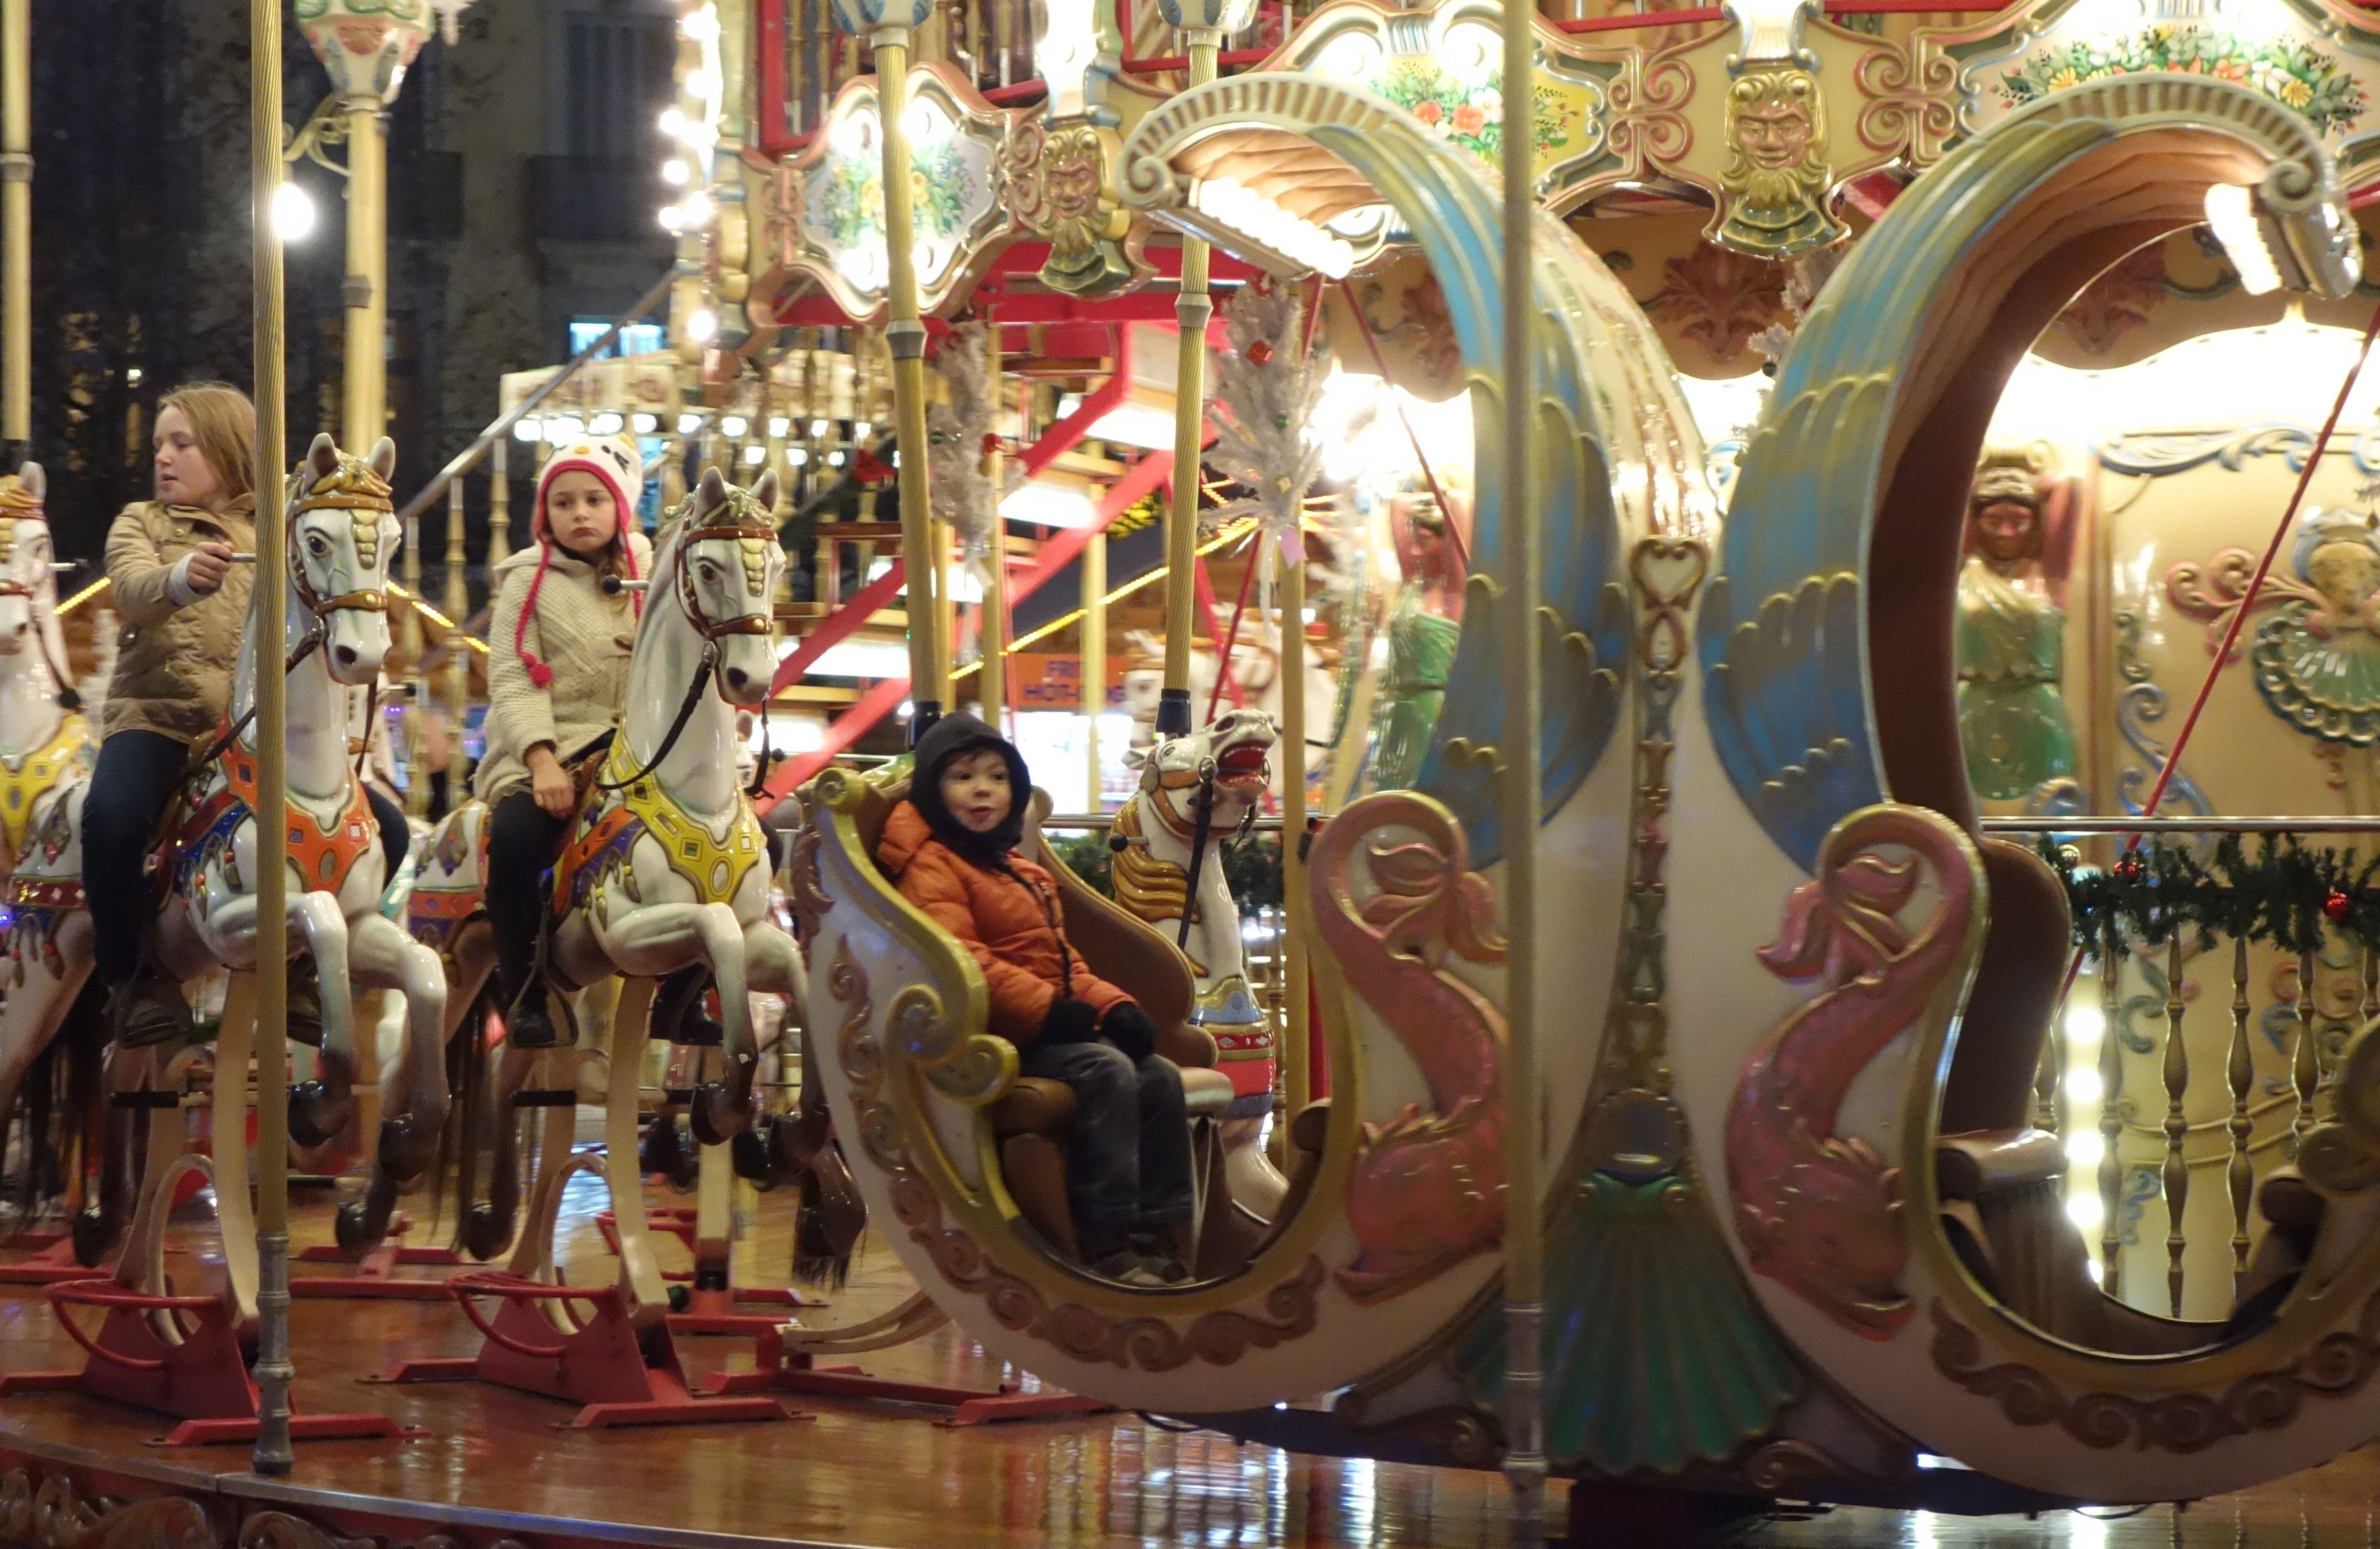
\includegraphics[width=\linewidth,height=\textheight,keepaspectratio,bb= 0 0 1106 720]{/home/mkg/Dropbox/images/DSC02910.JPG}
\clearpage
\onecolumn
\noindent Merry-go-round on the boardwalk in Tel Aviv, Israel.
\begin{lstlisting}
Filename: DSC09755.JPG

Date: 2016:04:06 13:12:31
Make: SONY
Model: DSC-RX100
Focal length (35mm eq): 28
Exposure: 0.03333333333333333
F stop: 1.8
ISO: 800
Width: 5470
Height: 3644
\end{lstlisting}
\clearpage

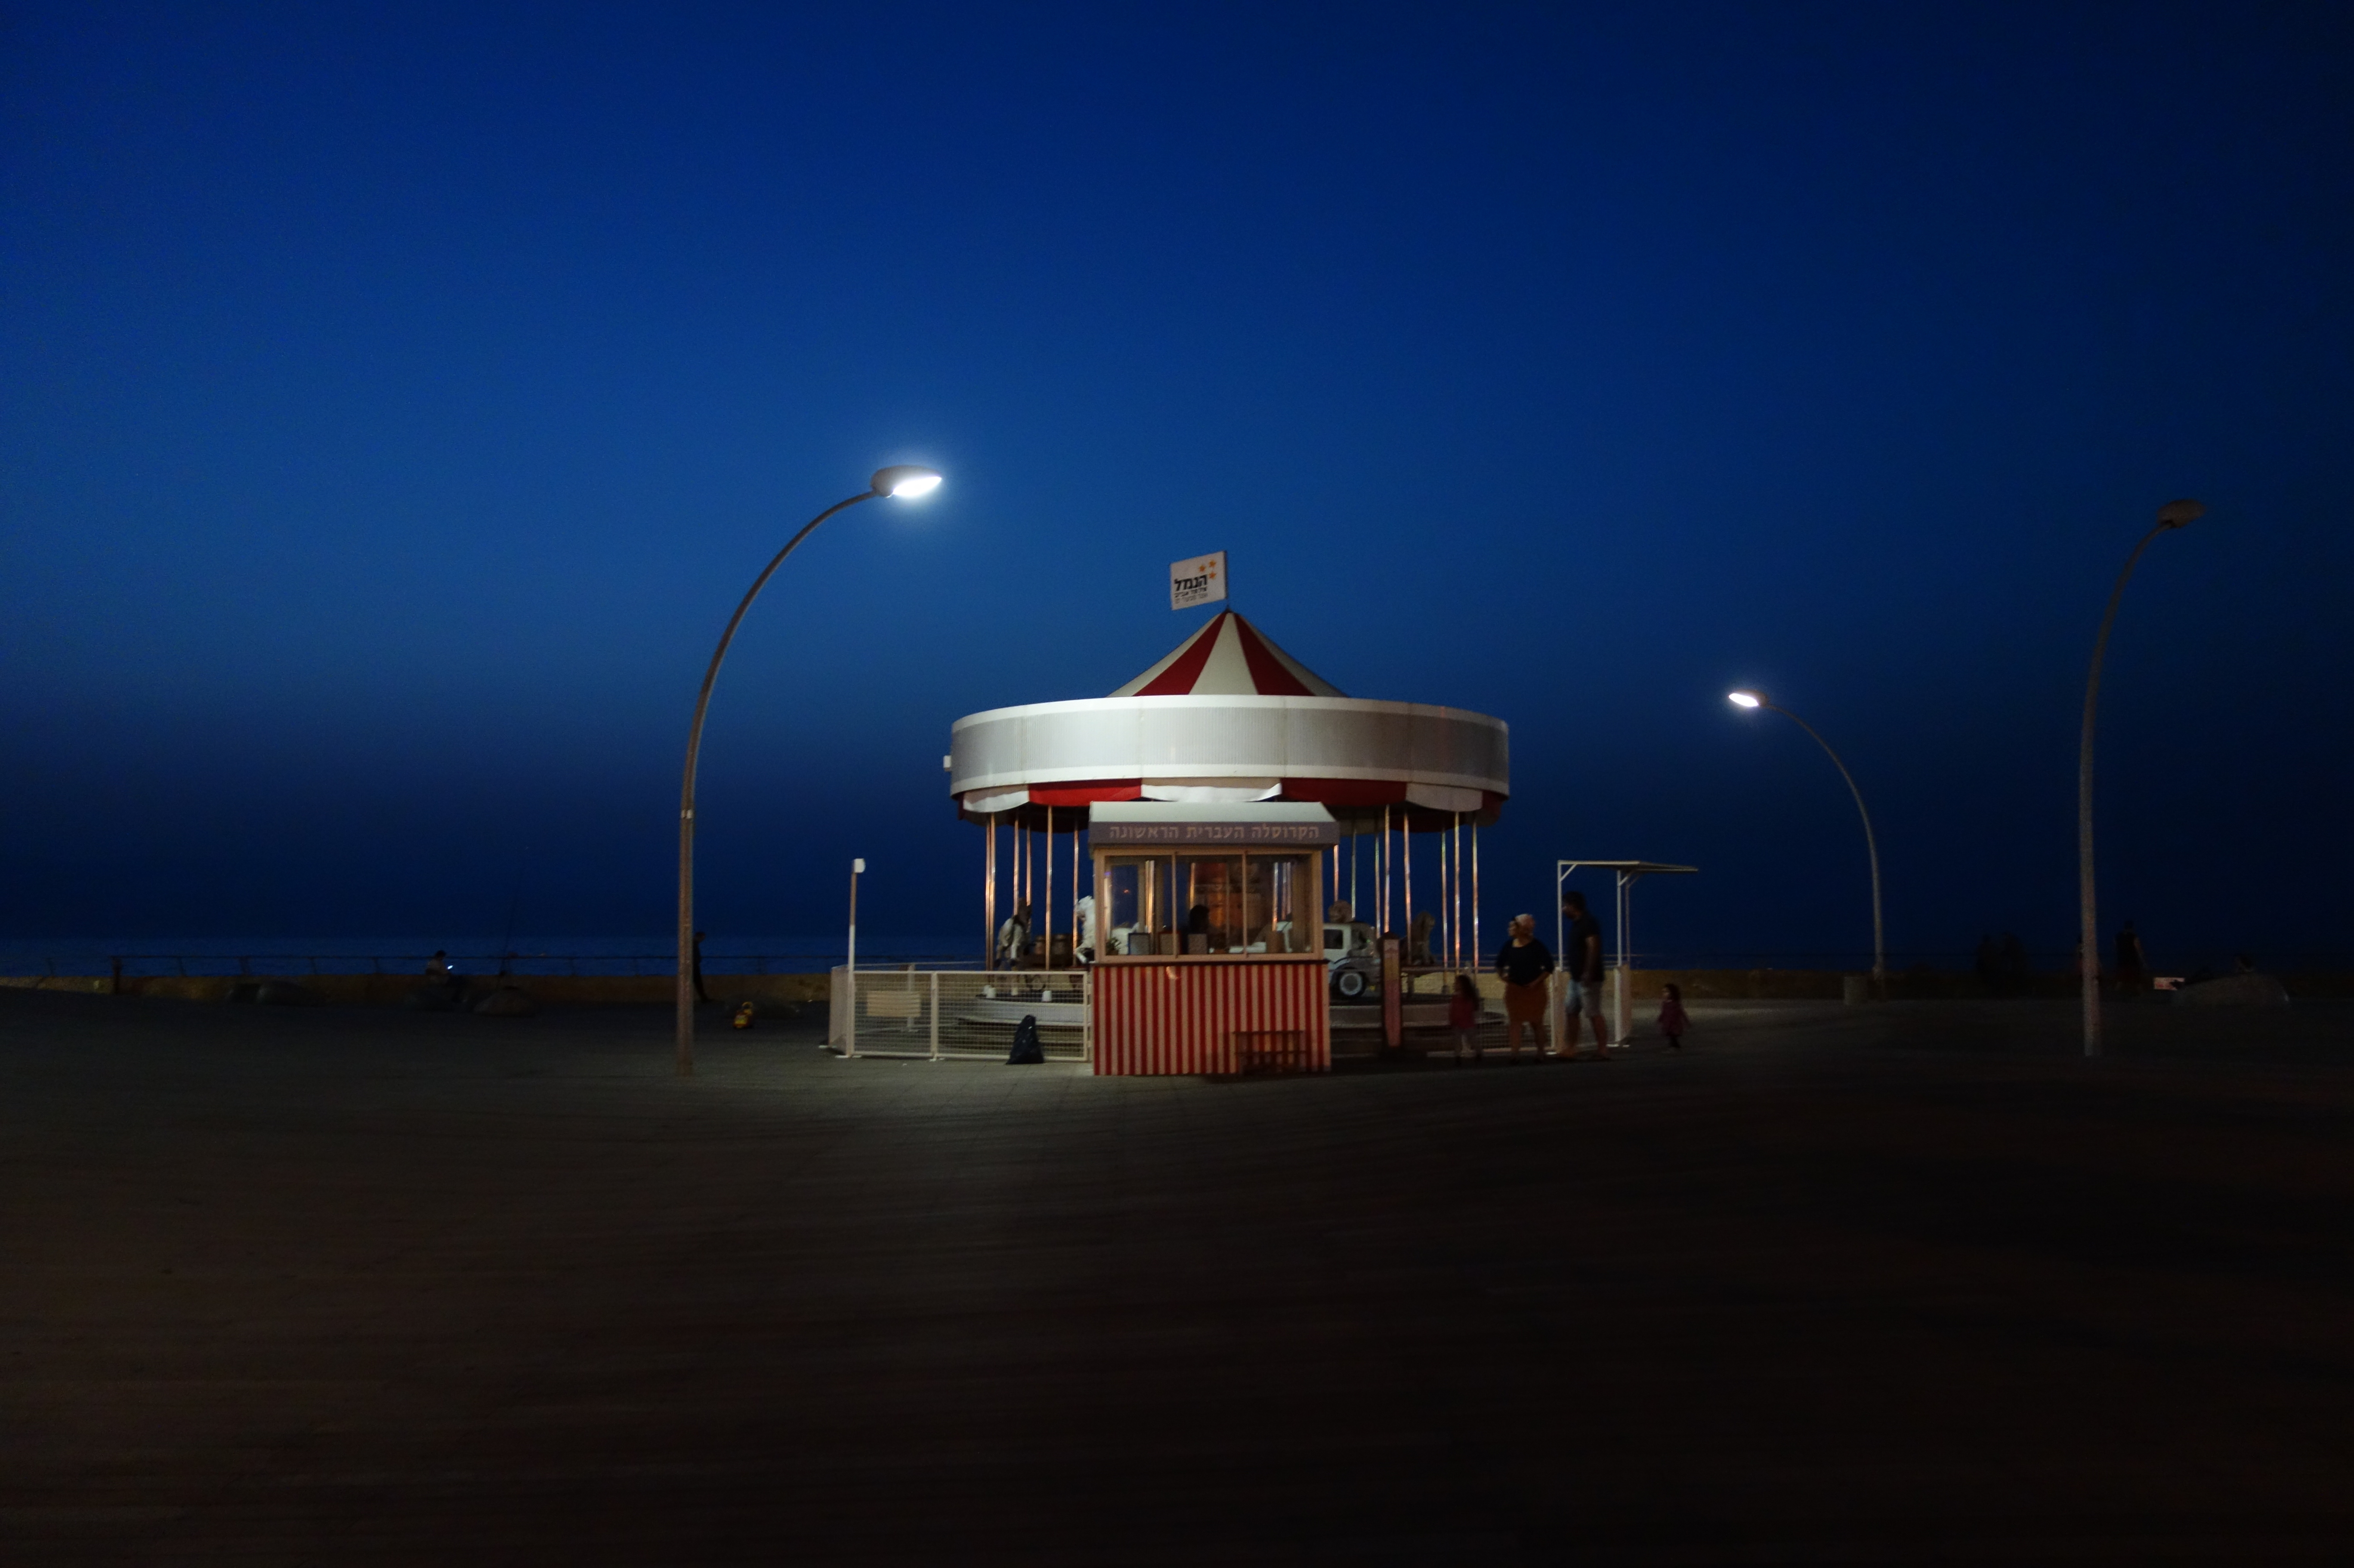
\includegraphics[width=\linewidth,height=\textheight,keepaspectratio,bb= 0 0 1125 750]{/home/mkg/Dropbox/images/DSC09755.JPG}
\clearpage
\onecolumn
\noindent A remnant of Music Row in Manhattan.
\begin{lstlisting}
Filename: 20130604_134331.jpg

Date: 2013:06:04 13:43:30
Make: SAMSUNG
Model: SGH-M919
Focal length (35mm eq): 31
Exposure: 0.002506265664160401
F stop: 2.2
ISO: 50
Width: 4128
Height: 2322
\end{lstlisting}
\clearpage

\includegraphics[width=\linewidth,height=\textheight,keepaspectratio,bb= 0 0 4128 2322]{/home/mkg/Dropbox/images/20130604_134331.jpg}
\clearpage
\onecolumn
\noindent Central Park, Manhattan.
\begin{lstlisting}
Filename: 20130619_080155.jpg

Date: 2013:06:19 22:01:54
Make: SAMSUNG
Model: SGH-M919
Focal length (35mm eq): 31
Exposure: 0.004273504273504274
F stop: 2.2
ISO: 50
Width: 4128
Height: 2322
\end{lstlisting}
\clearpage

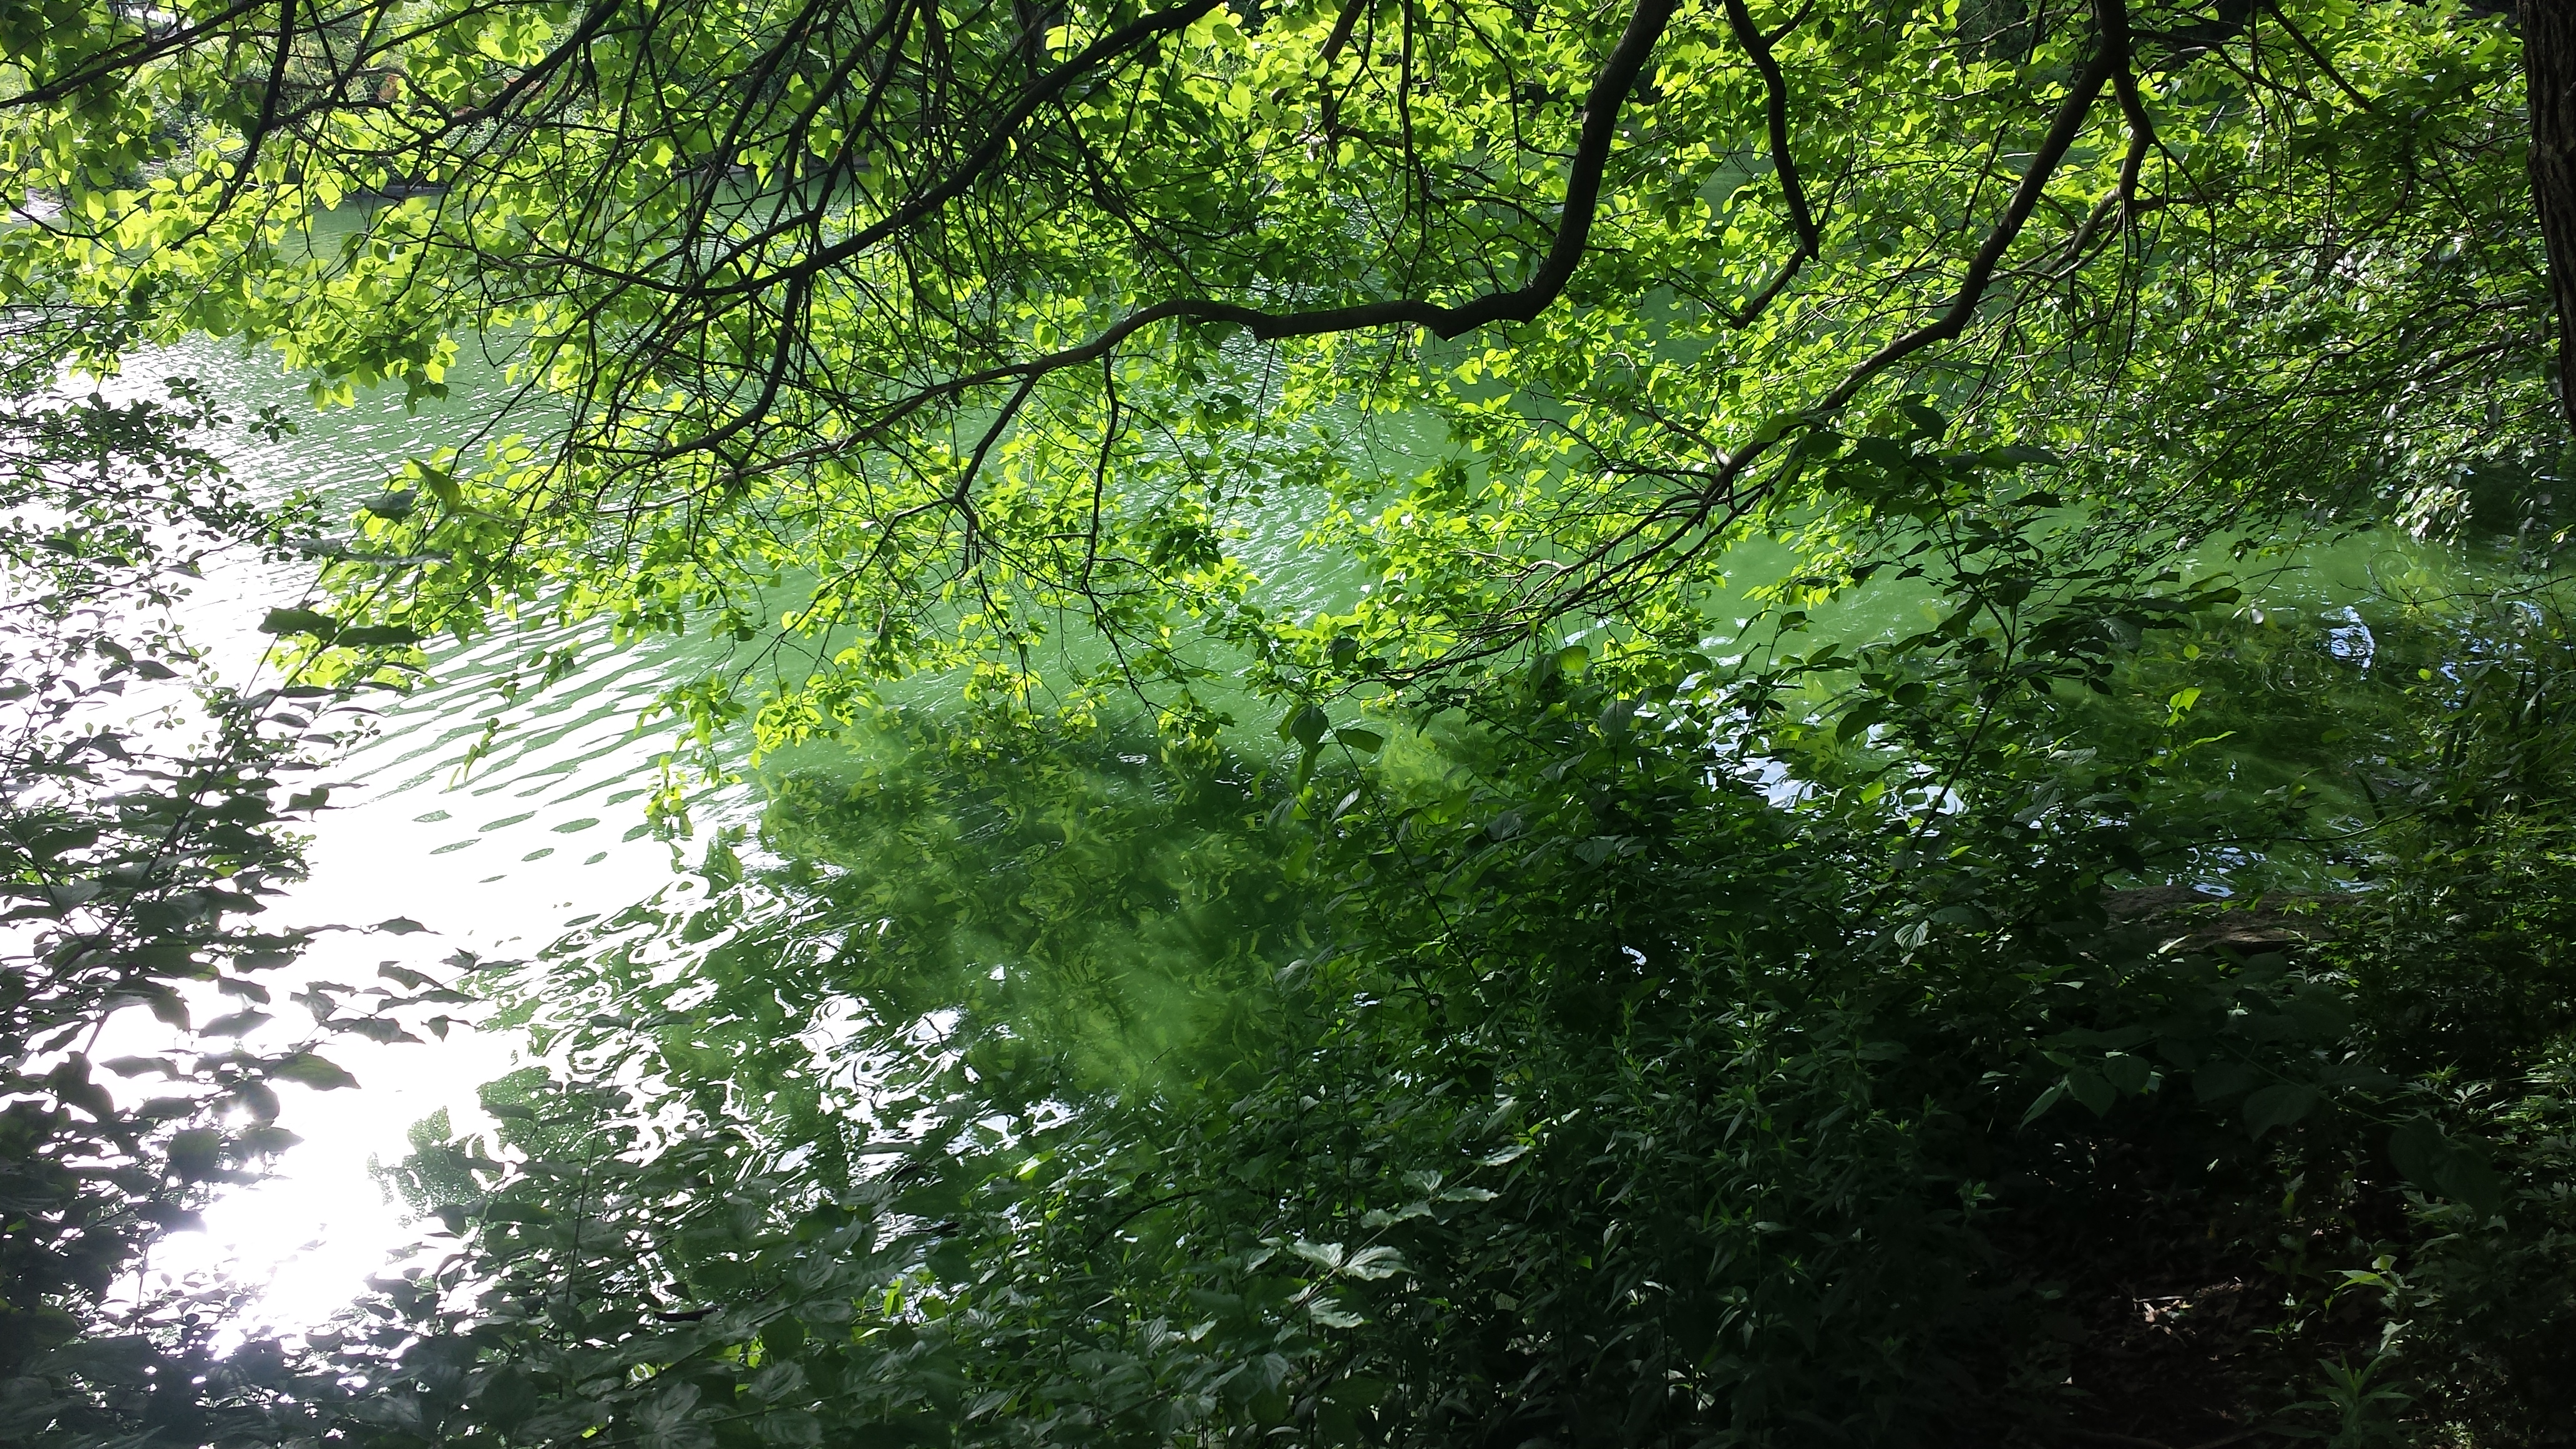
\includegraphics[width=\linewidth,height=\textheight,keepaspectratio,bb= 0 0 4128 2322]{/home/mkg/Dropbox/images/20130619_080155.jpg}
\clearpage
\onecolumn
\noindent My wife Heidi, in Central Park, New York City, before we were married.
\begin{lstlisting}
Filename: Heidi_in_Central_Park.jpg

Make: 
Model: 
ISO: ()
Width: 2147
Height: 3186
\end{lstlisting}
\clearpage

\includegraphics[width=\linewidth,height=\textheight,keepaspectratio,bb= 0 0 64 96]{/home/mkg/Dropbox/images/Heidi_in_Central_Park.jpg}
\clearpage
\onecolumn
\noindent Recoleta, Buenos Aires, Argentina.
\begin{lstlisting}
Filename: SM-950U/20180216_201359.jpg

Date: 2018:02:16 20:13:59
GPS longitude: (58.0, 23.0, 19.699)
GPS latitude: (34.0, 35.0, 41.0521)
Make: samsung
Model: SM-N950U
Focal length (35mm eq): 26
Exposure: 0.1
F stop: 1.7
ISO: 1250
Width: 4032
Height: 3024
\end{lstlisting}
\clearpage

\includegraphics[width=\linewidth,height=\textheight,keepaspectratio,bb= 0 0 4032 3024]{/home/mkg/Dropbox/images/SM-950U/20180216_201359.jpg}


\end{document}

